\section{Introduction au Calcul Haute Performance (HPC)}\label{sec:hpc_intro}


\subsection{Le calcul scientifique et la simulation numérique}
%%%%%%%%%%%%%%%%%%%%%%%%%%%%%%%%%%%%%%%%%%%%%%%%%%%%%%%%%%%%%%

    À l'origine, les scientifiques observaient la nature et émettaient des théories pour expliquer leurs observations (voir \autoref{fig:edl_simu_new}). En se basant sur ces théories, ils réalisaient des expériences physiques pour les valider ou non. Ils faisaient alors de nouvelles expériences pour affiner leur théorie. Les simulations numériques sont alors apparues comme des alternatives aux expériences physiques qui étaient souvent longues et onéreuses (voir \autoref{fig:edl_simu_new}). Des scientifiques comme Pythagore réalisaient ces simulations en faisant des calculs manuels ou en s'aidant de tables précalculées. Du fait de la limitation de leur capacité de calcul et de temps disponible, c'est avec l'apparition de l'informatique que les simulations sont devenues réellement exploitables.
    
    
    \begin{figure}[t!]
        \centering
        \begin{subfigure}[t]{0.48\textwidth}
            \centering
            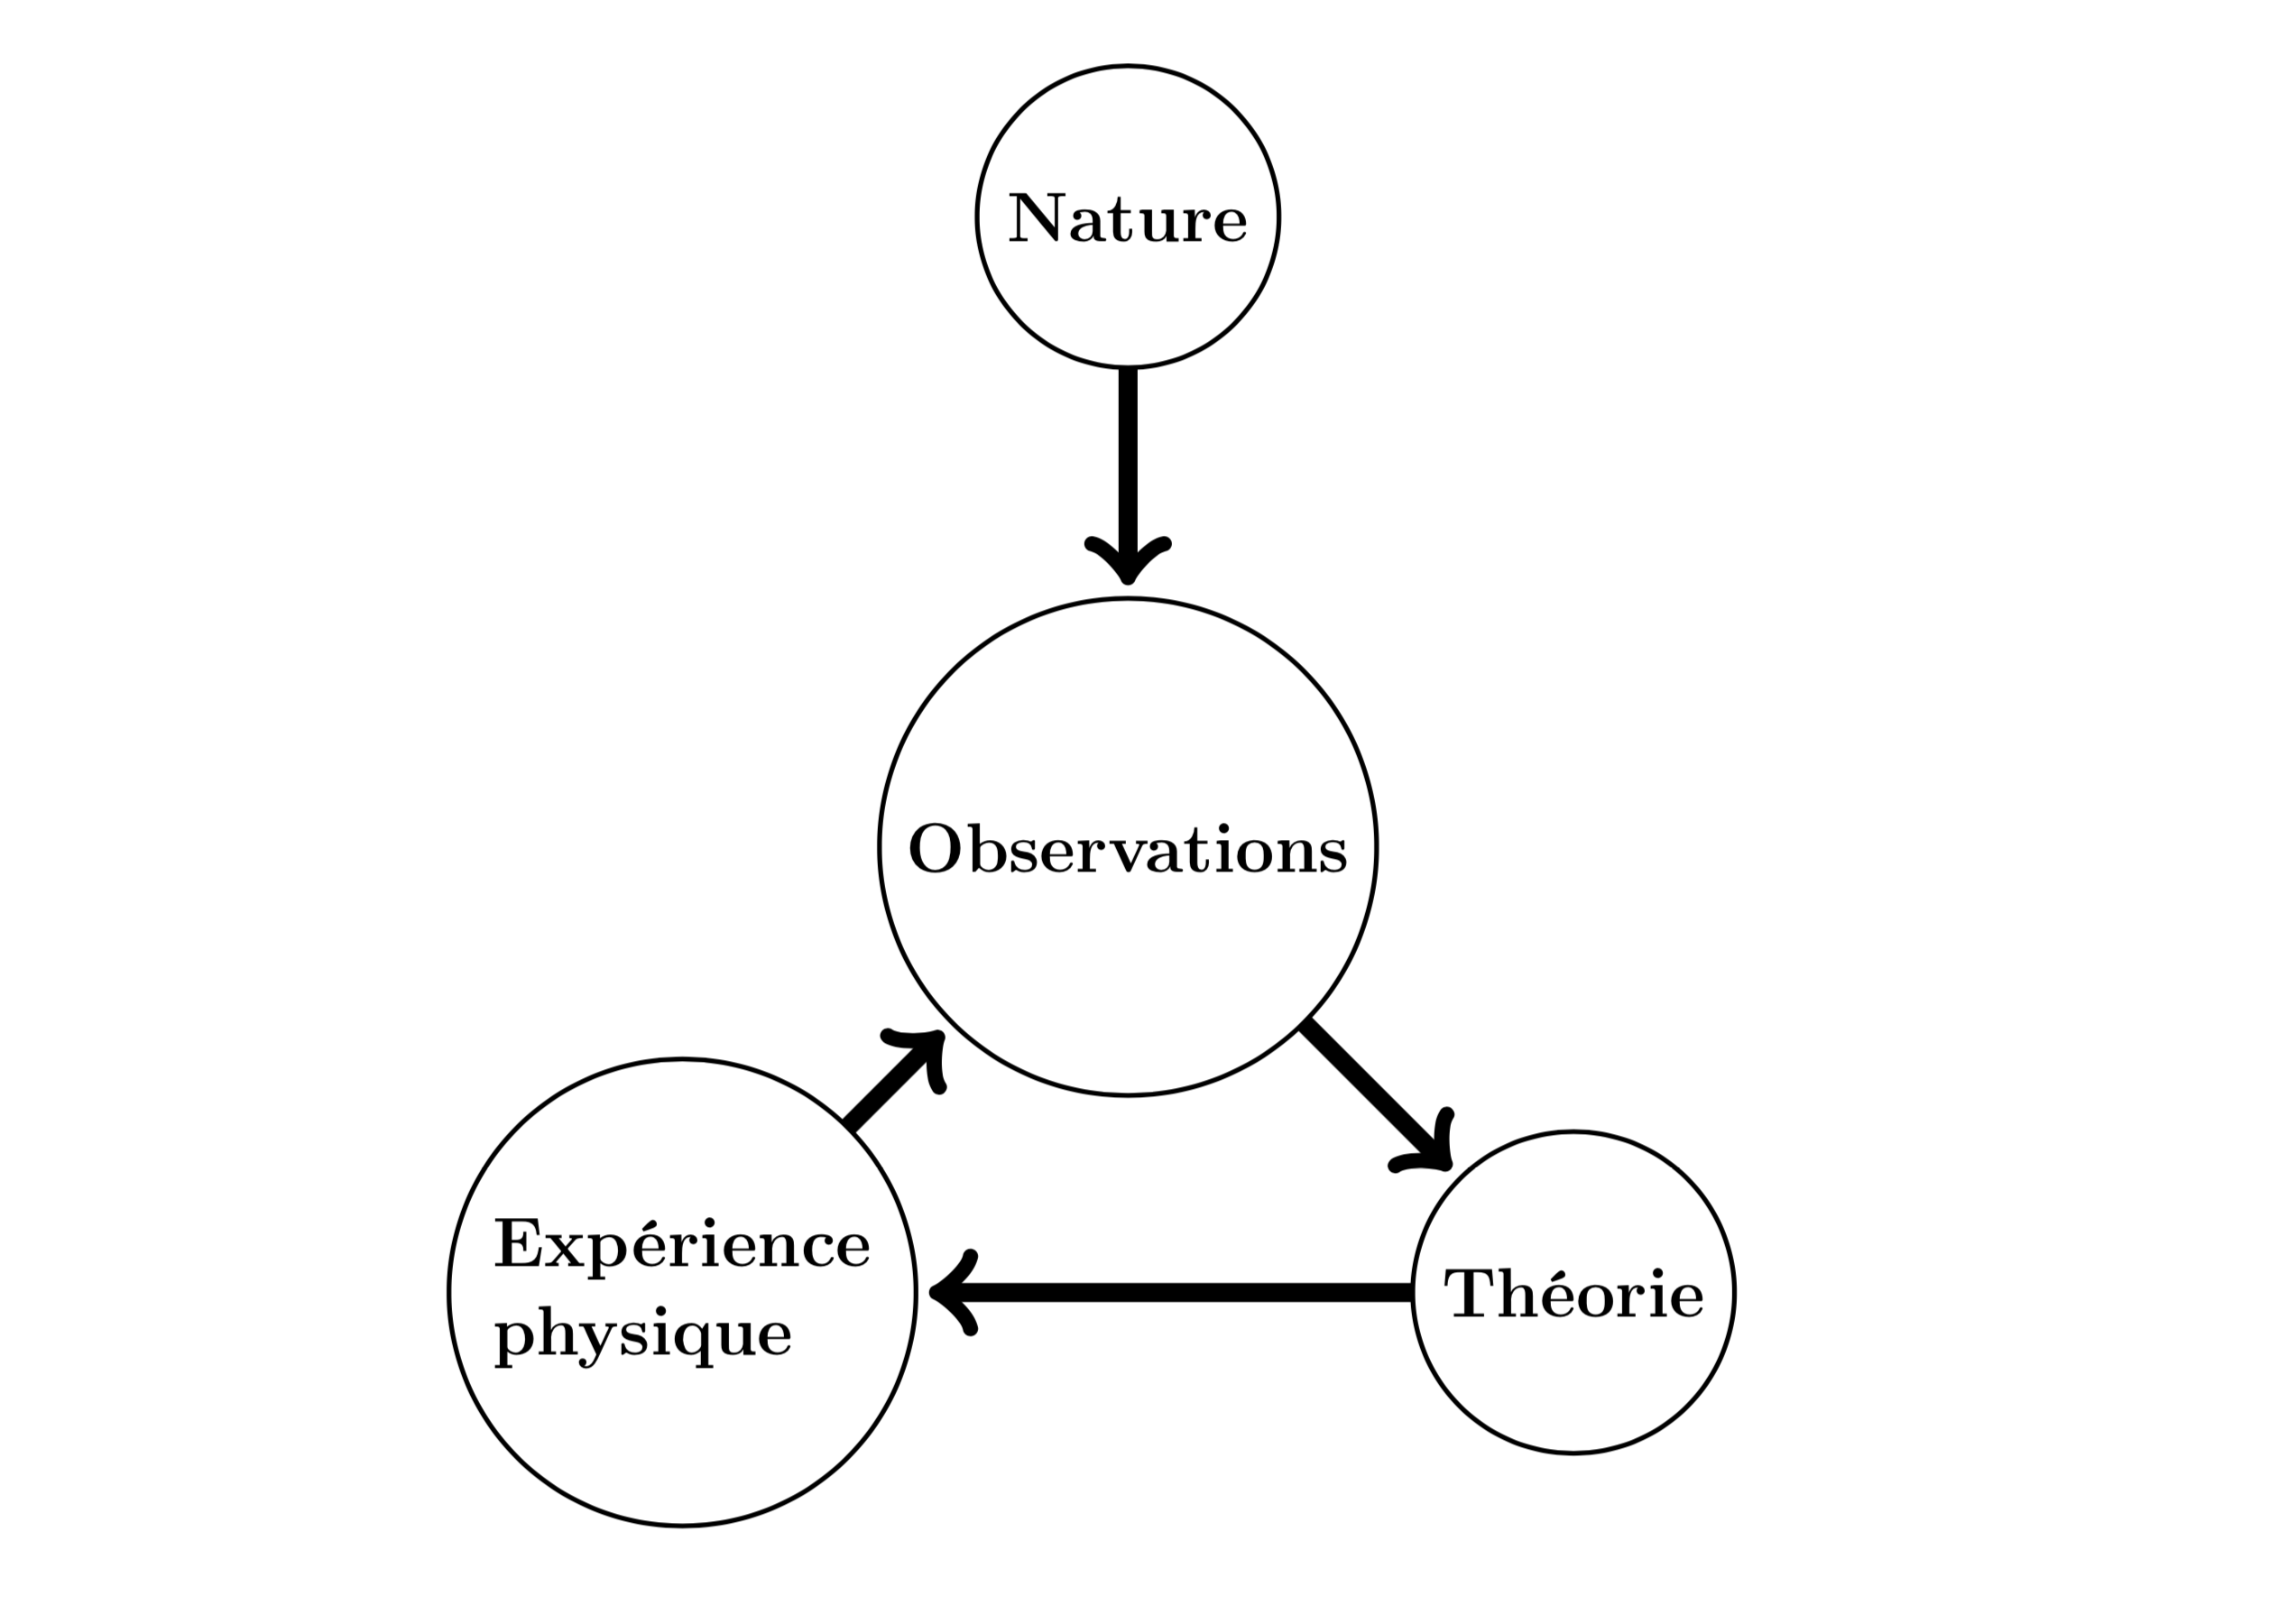
\includegraphics[width=\linewidth]{images/edl_simu_old.png}
            \caption{\label{fig:edl_simu_old}Les expériences physiques permettent de valider les théories.}
        \end{subfigure}\hfill
        \begin{subfigure}[t]{0.48\textwidth}
            \centering
            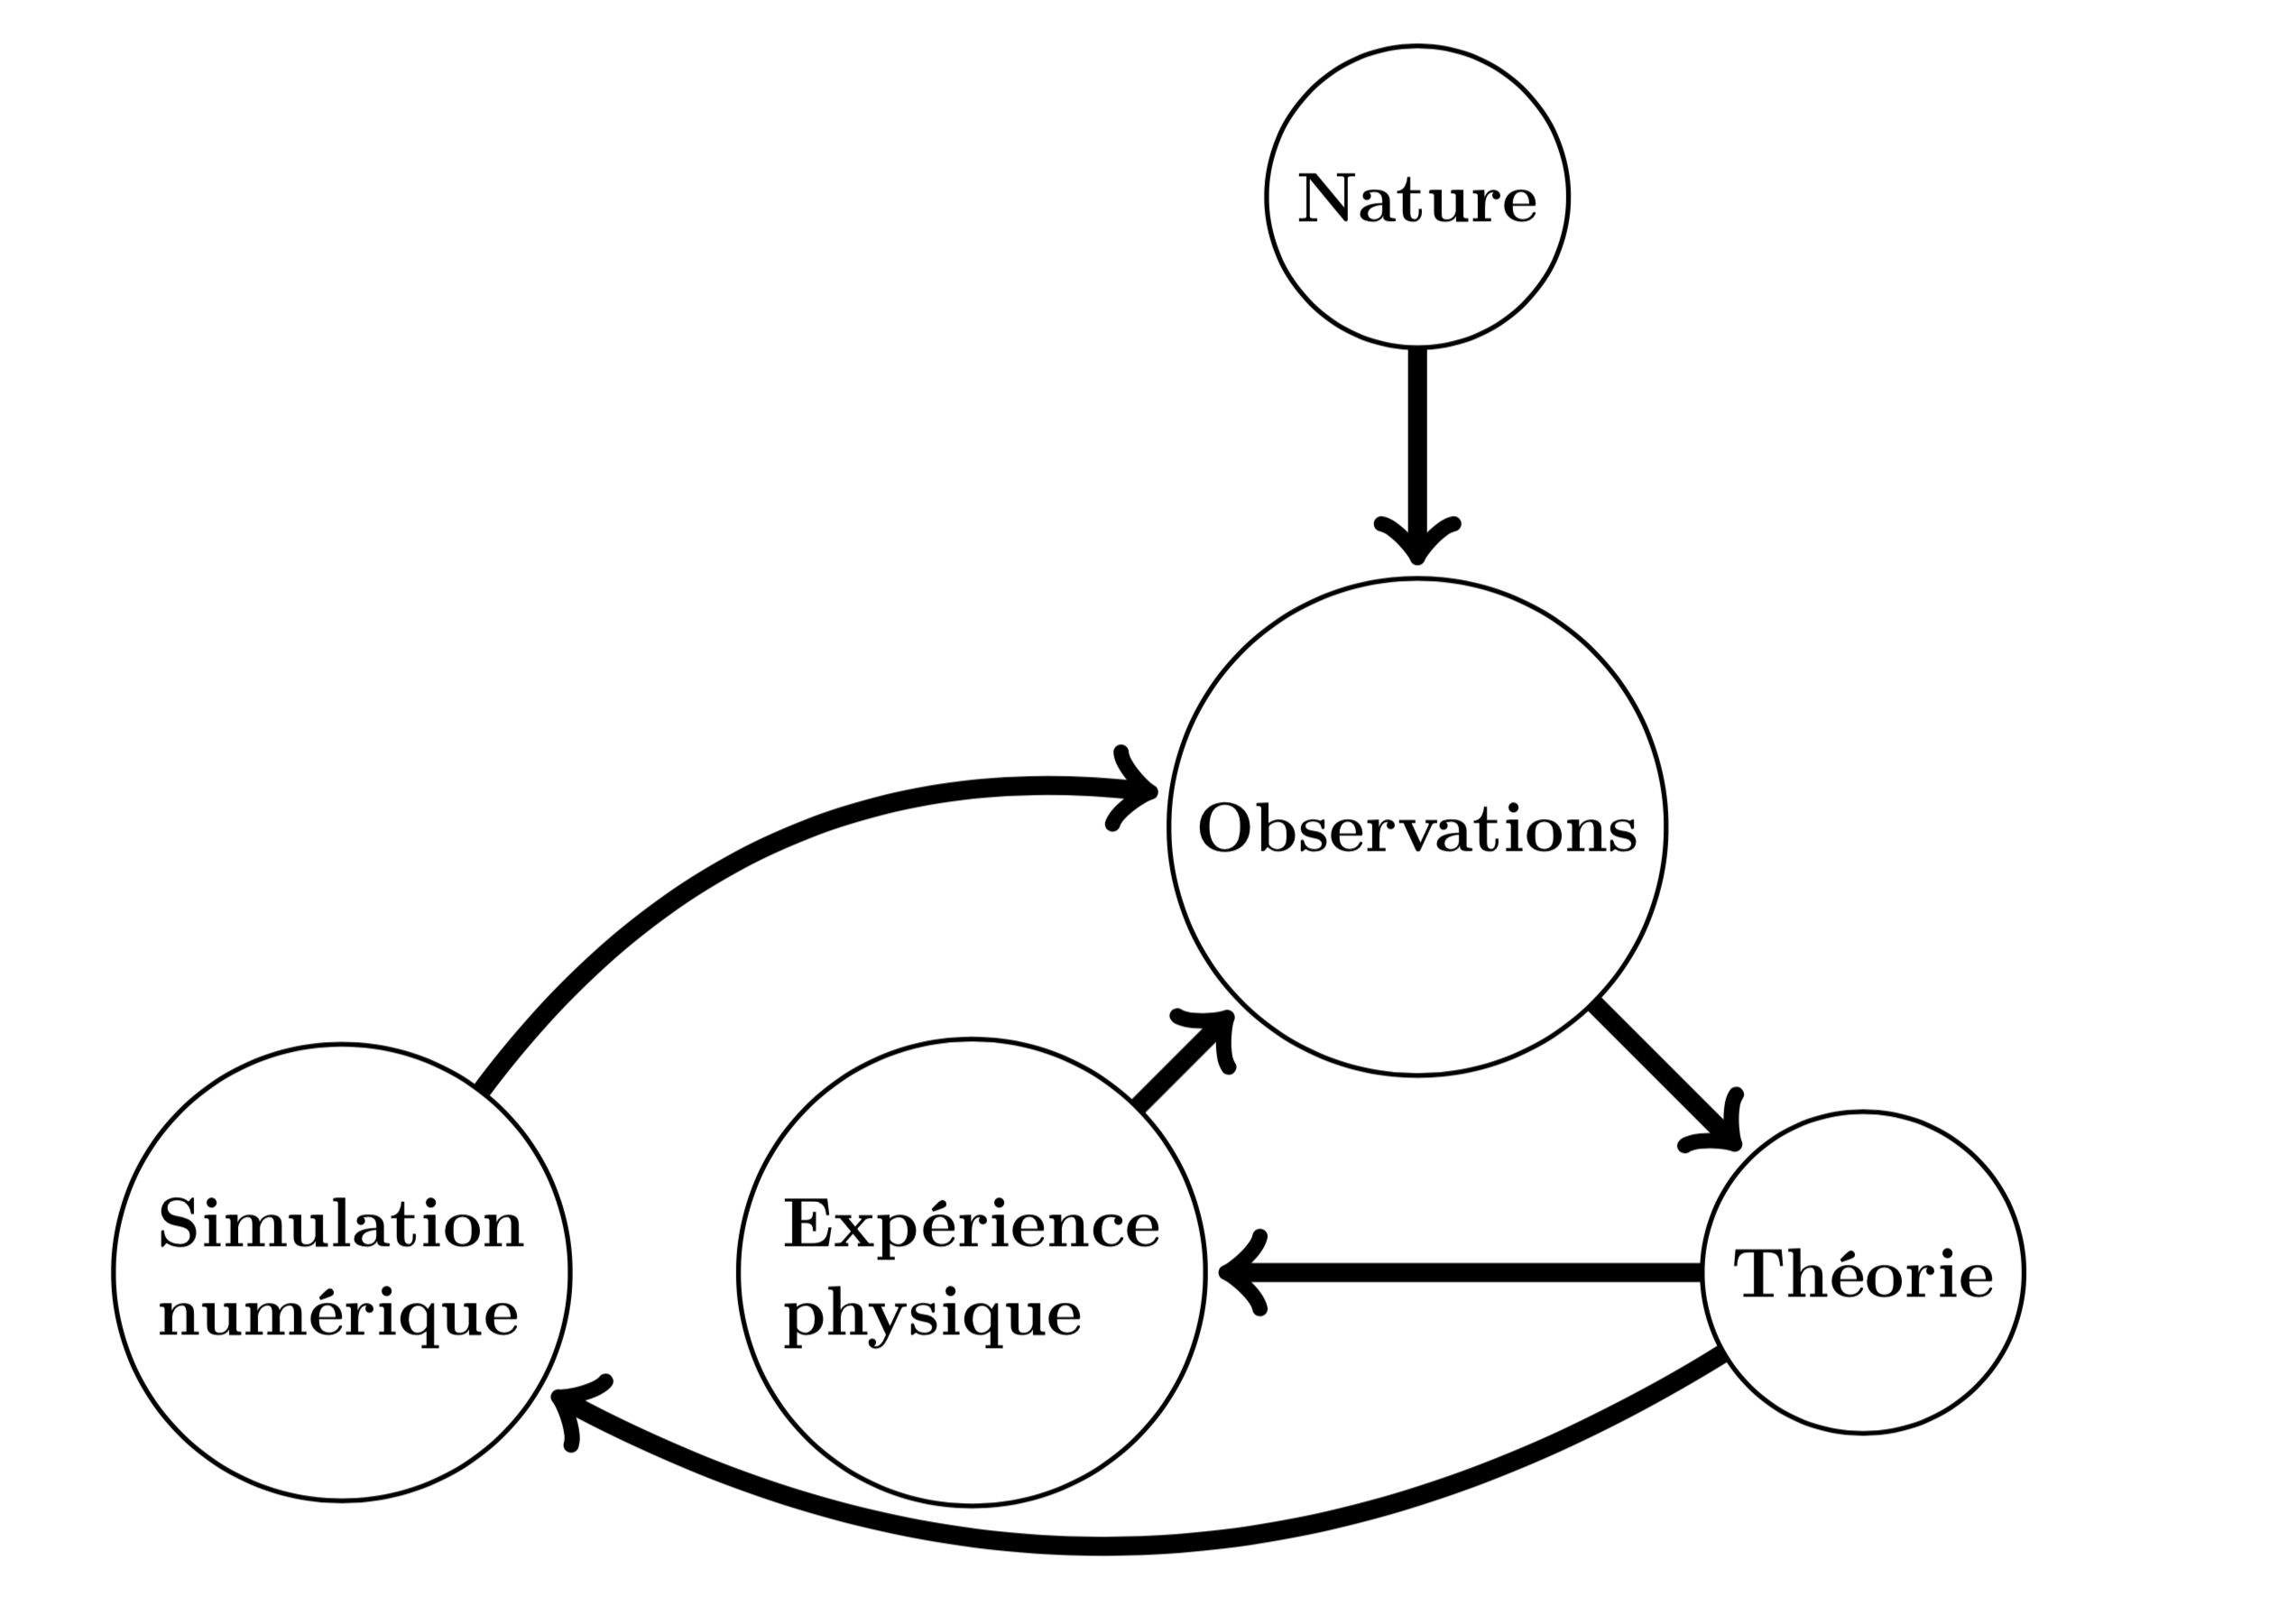
\includegraphics[width=\linewidth]{images/edl_simu_new.png}
            \caption{\label{fig:edl_simu_new}La simulation numérique peut être une alternative aux expériences physique.}
        \end{subfigure}
        \caption{La simulation numérique a apporté une nouvelle façon d'expérimenter les théories.}
        \label{fig:tikz_simulation}
    \end{figure}
    

      
    %TikZ picture
%\begin{figure}
%\begin{center}
%\begin{minipage}[]{.5\textwidth}
%\begin{tikzpicture}[->,shorten >=1pt,auto,node distance=3.8cm,   scale=0.49, every %node/.style={transform shape}]
%\tikzstyle{every state}=[fill=none,draw=black,text=black,  , font=\bf]
%\tikzstyle{edge_style} = [draw=black, line width=2, ultra thick]
%\tikzstyle{node_style} = [circle,draw=blue,fill=blue!20!,font=\sffamily\Large\bfseries]
%\node[state]					    (A)                     {Nature};
%\node[state]        				(B) [below of=A]        {Observations};
%\node[state,]         		    (D) [below right of=B]  {Théorie};
%\node[state, align=left]         	(C) [below left of=B]   {Expérience\\ physique};
%\path
%(A) edge [edge_style]   node {} (B)
%(B) edge [edge_style]   node {} (D)
%(C) edge [edge_style]   node {} (B)
%(D) edge [edge_style]   node {} (C);
%\end{tikzpicture}
%\end{minipage}%
%\begin{minipage}[]{.5\textwidth}
%\begin{tikzpicture}[->,shorten >=1pt,auto,node distance=3.8cm,   scale=0.49, every %node/.style={transform shape}]
%\tikzstyle{every state}=[fill=none,draw=black,text=black,  , font=\bf]
%\tikzstyle{edge_style} = [draw=black, line width=2, ultra thick]
%\tikzstyle{node_style} = [circle,draw=blue,fill=blue!20!,font=\sffamily\Large\bfseries]
%\node[state]					(A)                    {Nature};
%\node[state]        					(B) [below of=A] {Observations};
%\node[state,]         					(D) [below right of=B] {Théorie};
%\node[state, align=left]         	(C) [below left of=B] {Expérience\\ physique};
%\node[state, align=left]        	(E) [left of=C]       {Simulation\\numérique};
%\path
%(A) edge [edge_style]            node {} (B)
%(B) edge [edge_style]     node {} (D)
%(C) edge [edge_style]           node {} (B)
%(D) edge [edge_style]             node {} (C)
%edge [edge_style, bend left]     node {} (E)
%(E) edge [edge_style, bend left]  node {} (B);
%\end{tikzpicture}
%\end{minipage}
%\end{center}
%\caption{La simulation numérique a apporté une nouvelle façon d'expérimenter les théories.} 
%\label{fig:tikz_simulation}
%\end{figure} 
     
    
     
    \subsubsection{Principe de la simulation numérique}
    %%%%%%%%%%%%%%%%%%%%%%%%%%%%%%%%%%%%%%%%%%%%%%%%
    
        La majorité des simulations numérique sont basées sur des équations dites \textit{gouvernantes} et qui sont des approximations des phénomènes étudiés. Ces équations ont besoin d'être discrétisées pour pouvoir être exécutées par un ordinateur. En mathématiques, la discrétisation est un procédé qui permet de passer d'un modèle à son équivalent discret. Ce procédé ne permet pas de décrire le phénomène réel, mais de l'approcher avec plus ou moins d'erreurs. Pour améliorer ces simulations, ces représentations doivent utiliser des maillages les plus fins possible (voir \autoref{pic_maillage}). Une autre approche utilise des modèles probabilistes pour représenter un comportement. Elle est adaptée pour des phénomènes où chaque élément peut subir différents événements. Pour chaque étape du calcul, le résultat évolue grâce à des tirages aléatoires (méthode de Monte-Carlo \cite{Kroese2014}). Pour améliorer la précision des simulations, il est donc nécessaire d'augmenter le nombre de tirages et donc le nombre de calculs à réaliser.
        Que ce soit pour affiner la taille des maillages ou augmenter le nombre de tirages, les simulations numériques nécessitent de grandes puissances de calculs. 
            
            \begin{figure}
            \center
            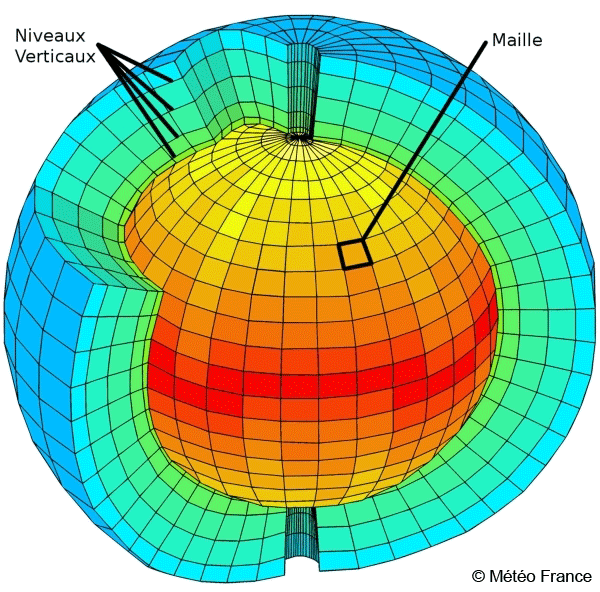
\includegraphics[width=5cm]{images/Chapitre1/maillage.png}
            \caption{\label{pic_maillage} Le maillage le plus fin exploité par Météo-France pour ses prévisions régionales restitue des mailles de 2,5 km de côté (source \url{www.irma-grenoble.com}).}
            \end{figure}

    
    \subsubsection{Quelques applications de simulations numériques}
    %%%%%%%%%%%%%%%%%%%%%%%%%%%%%%%%%%%%%%%%%%%%%%%%
        Lorsque l'on évoque la simulation numérique, on pense souvent aux domaines physiques (météorologie, mécanique, biologie), mais elle peut aussi être utilisée en sciences humaines (sociologie, analyse démographique) ou dans le domaine de la sécurité nationale. En effet, Alan Turing a développé les premiers ordinateurs lors de la fin de la Deuxième Guerre mondiale pour aider au décryptage des messages allemands. En 1936, il avait présenté les premiers concepts de programmes et donné naissance à l'aide d'une expérience de pensée à l'ancêtre des ordinateurs nommée machine de Turing.  L'utilisation de simulations numériques a de nombreux avantages. En plus de profiter de la puissance de calculs des ordinateurs, elle permet de simuler des phénomènes dont les conditions ne sont pas reproductibles sur terre (physique théorique). Un autre avantage est de réduire drastiquement les coûts d'une expérience, par exemple pour la réalisation de crash automobile, où ce ne sont plus de réels modèles de voiture, mais bien des voitures virtuelles qui sont crashées sur des murs.
        
        Dans le domaine de la santé, l'étude de la structure des protéines est primordiale.  Ces molécules qui assurent les fonctions élémentaires d'une cellule interviennent dans la majorité des processus biologiques (régulation du métabolisme, défense immunitaire). Dans ce genre de simulation, le pas de temps est de l'ordre de la nanoseconde. Grâce à la simulation numérique, une meilleure compréhension de ces molécules permet la découverte de nouveaux médicaments ou antibiotiques. 
        Aussi, des modélisations peuvent être utilisées pour analyser la propagation d'un virus comme la grippe aviaire à l'échelle mondiale pour mieux protéger les populations\cite{CEA2007}. En février 2020, le gouvernement français indiquait travailler sur la modélisation de la propagation du COVID-19\footnote{\url{https://www.gouvernement.fr/info-coronavirus}} (coronavirus). Cette modélisation fait intervenir plusieurs paramètres comme le lieu et la période d'incubation du virus ou encore la fréquentation et les destinations des passagers des 4000 principaux aéroports mondiaux. En mars 2020, le supercalculateur le plus puissant au monde (Summit) était utilisé pour identifier 77 molécules potentiellement efficaces contre le COVID-19 \cite{Smith2020}.

        En astrophysique, la simulation numérique est aussi capitale du fait de la non-reproductibilité des expériences en laboratoire.  À l'opposé de l'exemple précédent sur les protéines, elle permet d'étudier des objets aussi grands que complexes comme le système solaire, les galaxies ou bien l'univers. La simulation permet alors de faire évoluer le système avec un pas de temps allant jusqu'au million d'années. Une équipe du CEA a pu reconstituer le passé de la galaxie Andromède en analysant les observations réalisées grâce au satellite infrarouge Spitzer\cite{Block2006}. Après avoir mis au point le modèle adéquat et après plusieurs heures de simulation, ils ont pu déterminer qu'elle avait été percutée par une galaxie voisine il y a plus de 210 millions d'années et que sa forme actuelle résultait de cet impact (voir\autoref{pic:cea_galaxy}).
    
        
        \begin{figure}
            \center
            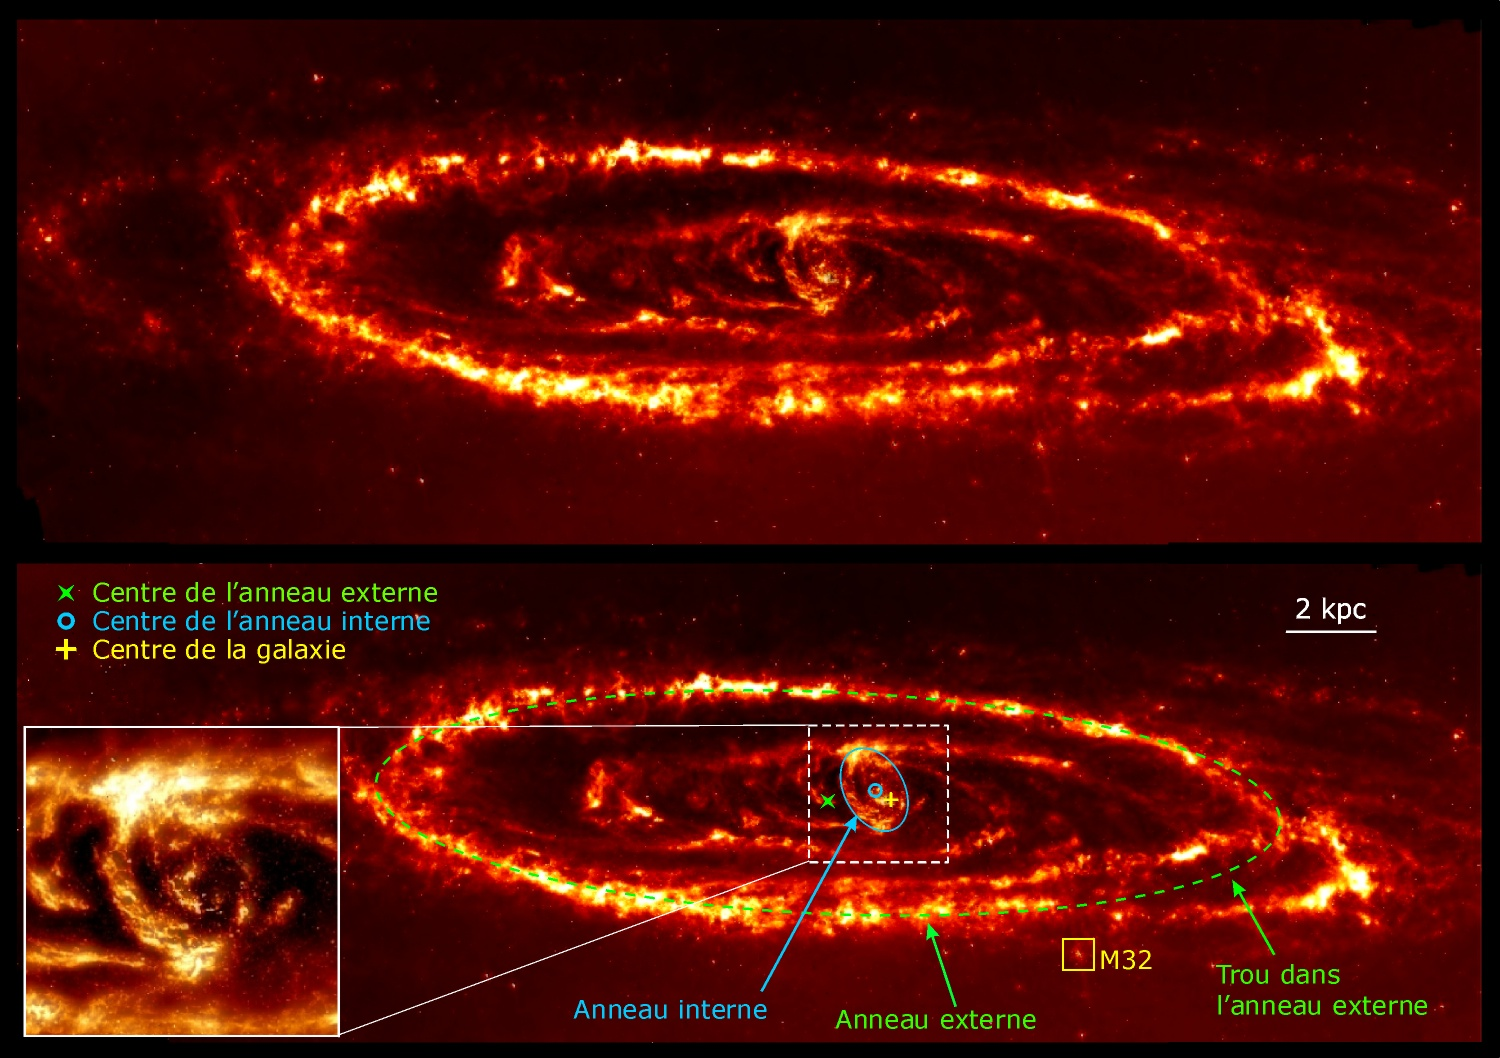
\includegraphics[width=12cm]{images/cea_galaxy.jpg}
            \caption{\label{pic:cea_galaxy} Cartographie de l'émission infrarouge des poussières  obtenues à l'aide du satellite Spitzer\protect\footnotemark. En bas : identification de la structure en double-anneau décentré et agrandissement de l'anneau interne. À la distance de M31, l'anneau interne a une dimension de 3 par 4.5 milliers d'années-lumière.}
        \end{figure}
        \footnotetext{\url{http://irfu.cea.fr/Phocea/Vie_des_labos/Ast/ast.php?id_ast=958&t=actu}}

        Pour la compétitivité et l'innovation des entreprises, les simulations numériques sont désormais un outil indispensable. Cet outil les aide à la conception, à la décision et au contrôle de leurs activités. 
        Dans l'industrie des hydrocarbures, la recherche pétrolière est très coûteuse : le coût d'un forage d'exploration maritime peut atteindre 100 millions d'euros\footnote{\url{https://www.planete-energies.com/fr/medias/decryptages/la-difficile-decision-de-lancer-un-forage}}.  Les pétroliers utilisent la simulation numérique pour analyser les fonds marins, modéliser les réservoirs de pétrole et, in fine, optimiser l'extraction du pétrole. Pour cela, ils utilisent des bateaux tractant d'immenses lignes flottantes pourvues de capteurs. Le principe est d'émettre des explosions, et d'analyser le réfléchissement des signaux sur le fond marin (voir \autoref{pic:hpl_petrole}). Grâce à l'analyse de ces données, il est alors possible de construire une cartographie du fond marin et ainsi déceler la présence ou non de réservoirs d'hydrocarbures.  En perçant le puits de façon optimale, il sera d'autant mieux exploité. De plus, le risque de forer au mauvais endroit est lui aussi diminué. Actuellement, le taux de succès est de deux forages sur trois.

        \begin{figure}
            \center
            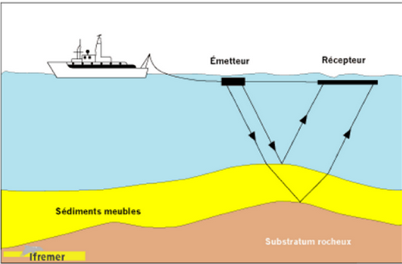
\includegraphics[width=8cm]{images/hpl_petrole.png}
            \caption{\label{pic:hpl_petrole}Étude de fond marin grâce à la sismique de réflexion.}
        \end{figure}


\subsection{Le calcul haute performance} \label{sec:supercomputer}
%%%%%%%%%%%%%%%%%%%%%%%%%%%%%%%%%%%%%%%%%%%%%%%%%%%%%%%%%%%%%%
        
        
    Aujourd'hui, presque que tout ce que nous utilisons a été simulé, à un tel point que l’avancée de nos sociétés dépend de la puissance de calcul disponible pour réaliser ces simulations. La rapidité de l'exécution des simulations numériques dépend alors de la puissance de calcul disponible pour exécuter l’application. Le domaine du \gls{hpc} est le domaine informatique qui consiste à exécuter ces applications le plus efficacement possible sur une plateforme. Celle-ci peut être un simple ordinateur personnel ou un centre de calculs dédié. De telles infrastructures sont utilisées dans de nombreux domaines dont les principaux sont la simulation numérique, la cryptographie, l'analyse de données (\textit{big data}), l’intelligence artificielle ou la sécurité. En fonction des besoins des applications (puissance de calcul, espace mémoire, stockage), mais aussi des budgets alloués, des infrastructures adaptées sont développées:
    
   \begin{enumerate}
        \item \textbf{Le supercalculateur dédié} (\textit{dedicated supercomputer}) consiste à la création d'une architecture unique qui ne sera pas répliquée.  Le premier supercalculateur élaboré par Seymour Cray alors employé de l'entreprise Control Data (le CDC6600) utilisait une telle architecture. Il était alors l'ordinateur le plus puissant de la planète grâce à une mémoire de 131000 mots de 60 bits, une fréquence de 40 MHz et sa capacité calculatoire de $3.3 \times 10^6$ opérations par seconde. À titre de comparaison, l'ordinateur portable utilisé pour écrire ce manuscrit est capable d'exécuter plus de $10^9$ opérations par seconde. L'objectif de ce type d'infrastructure est d'être parfaitement adapté aux besoins de l'application. La conception de ces architectures étant unique, les frais de conception sont très élevés, mais cette spécificité en fait des architectures très performantes. 
        
        \item \textbf{Le commodity cluster}. L'augmentation de la vitesse des circuits ainsi que l'augmentation exponentielle du nombre de transistors des circuits a rendu les supercalculateurs dédiés très difficiles à alimenter en énergie ou à être refroidi. Il a alors fallu repenser leur architecture pour continuer à augmenter la puissance des supercalculateurs. Les \textit{commodity cluster} agrègent du matériel grand public (haut de gamme) pour former des grappes de calculs de plusieurs milliers de processeurs. La performance de ces architectures ne repose pas sur l'utilisation de matériels ultra-optimisés, mais sur l'agrégation de milliers de serveurs (noeuds de calculs) travaillant ensemble. L'Intel Paragon est un des premiers exemples de cluster construit par Intel en 1992\footnote{source: \url{https://www.top500.org/featured/systems/intel-xps-140-paragon-sandia-national-labs/\#Historical}}, qui regroupe 3680 processeurs indépendants atteignant une puissance cumulée de $143.40 \times 10^9$ \gls{FLOP}. Ce modèle de supercalculateur est le plus répandu actuellement et a permis l'élaboration des supercalculateurs les plus puissants de la planète. Ces infrastructures sont généralement développées pour des industries privées ou de grandes universités (voir \autoref{fig:hpc_bsc_super}).
        
        \item \textbf{L'informatique en nuage} (\textit{cloud computing}),  utilise le modèle \textit{System as a Service} (SAS) pour apporter aux entreprises manquant de moyens, ou de compétences, un accès à une infrastructure HPC externalisée. Les principaux avantages sont la flexibilité d'usage (adapter l'infrastructure à son besoin) ainsi que la sous-traitance de la gestion de la plateforme. L'informatique en nuage permet  à des petites structures (PME, petite université) d'avoir accès à une ressource de calculs facilement à des coûts modérés. Nous pouvons notamment citer le projet SIMSEO \cite{Saguez2016} qui a pour but de sensibiliser et d'accompagner les PME à utiliser la simulation numérique. %L'informatique en nuage permet aussi de faciliter les évolutions de matériels et permet d'utiliser les dernières technologies.
        %Le \textit{nuage} peut être implémenté de deux façons. La première est d'utiliser un nuage public où les machines sont gérées par le prestataire directement dans leur centre de données. La deuxième est d'installer un \textit{nuage} privé, \textbf{TODO} le client choisi où installer la plateforme. Cette seconde solution est particulièrement recherchée par les entreprises utilisant des données sensibles et refusant qu'elles soient stockées dans un autre pays. 
        
        \item \textbf{Les grilles informatiques} (\textit{Grid Computing}) sont un regroupement de ressources informatique à grande échelle (nationale voir internationale). Par exemple \textit{Einstein@Home} \cite{Abbott2009} est un projet de recherche mondial sur les ondes gravitationnelles  qui regroupe les ordinateurs de 50000 utilisateurs connectés à travers le monde pour analyser les données transcrites par des capteurs.
    \end{enumerate}
        
        
        \begin{figure}
        \center
        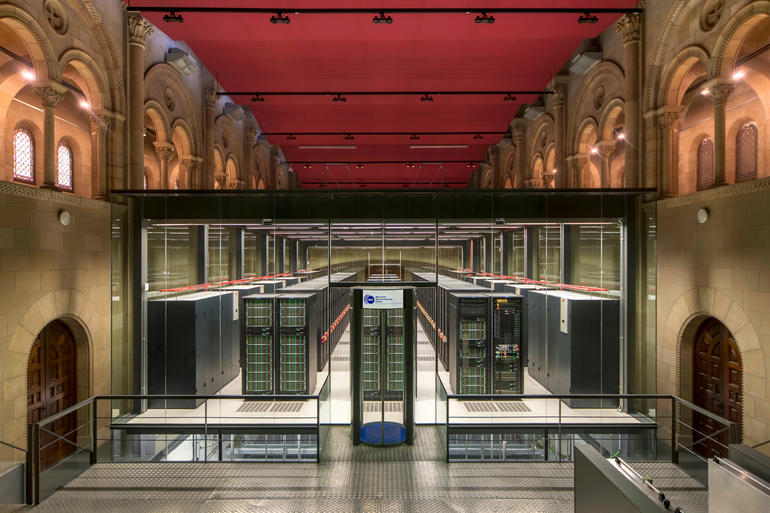
\includegraphics[width=12cm]{images/hpc_bsc_super.jpg}
        \caption{\label{fig:hpc_bsc_super} Le supercalculateur du Centre de Calcul de Barcelone (BSC) est installé dans une ancienne chapelle.}
        \end{figure}
        
        
    
        
    \subsubsection{Architecture des supercalculateurs}
    %%%%%%%%%%%%%%%%%%%%%%%%%%%%%%%%%%%%%%%%%%%%%%
    
        Les deux principales caractéristiques d'un supercalculateur sont sa capacité à calculer rapidement ainsi que sa capacité à mémoriser les informations et les résultats produits. L'architecture des supercalculateurs modernes n'est pas très différente de celle des ordinateurs classiques. La puissance d'une telle plateforme vient seulement de l'agrégation de centaines de ressources de calculs, capables de travailler ensemble pour résoudre un problème complexe. Le domaine du HPC consiste à exécuter efficacement des applications sur de telles architectures. Pour cela, l'infrastructure utilisée doit gérer l'équilibrage de la charge de calculs sur les différentes ressources disponibles ainsi que la gestion des communications entre les ressources. Un supercalculateur moderne possède généralement les cinq parties suivantes:
      
        \begin{enumerate}
        
            \item \textbf{Les serveurs} utilisés dans un supercalculateur possèdent un ou plusieurs processeurs. Comme un ordinateur classique, chaque processeur est relié à la mémoire et au stockage (voir \autoref{fig:motherboard}). En fonction des configurations, chaque serveur peut être agrémenté d'un ou plusieurs accélérateurs (GPU). La principale différence avec un ordinateur classique, autre que la puissance des matériels utilisés, vient du système d'interconnexion (voir \autoref{fig:dl360_back}). Les serveurs doivent pouvoir échanger des informations pour se synchroniser ou partager des résultats entre eux et accéder au stockage (voir \autoref{sec:edl_interco}).
        
                \begin{figure}[t!]
                    \centering
                    \begin{subfigure}[t]{0.48\textwidth}
                        \centering
                        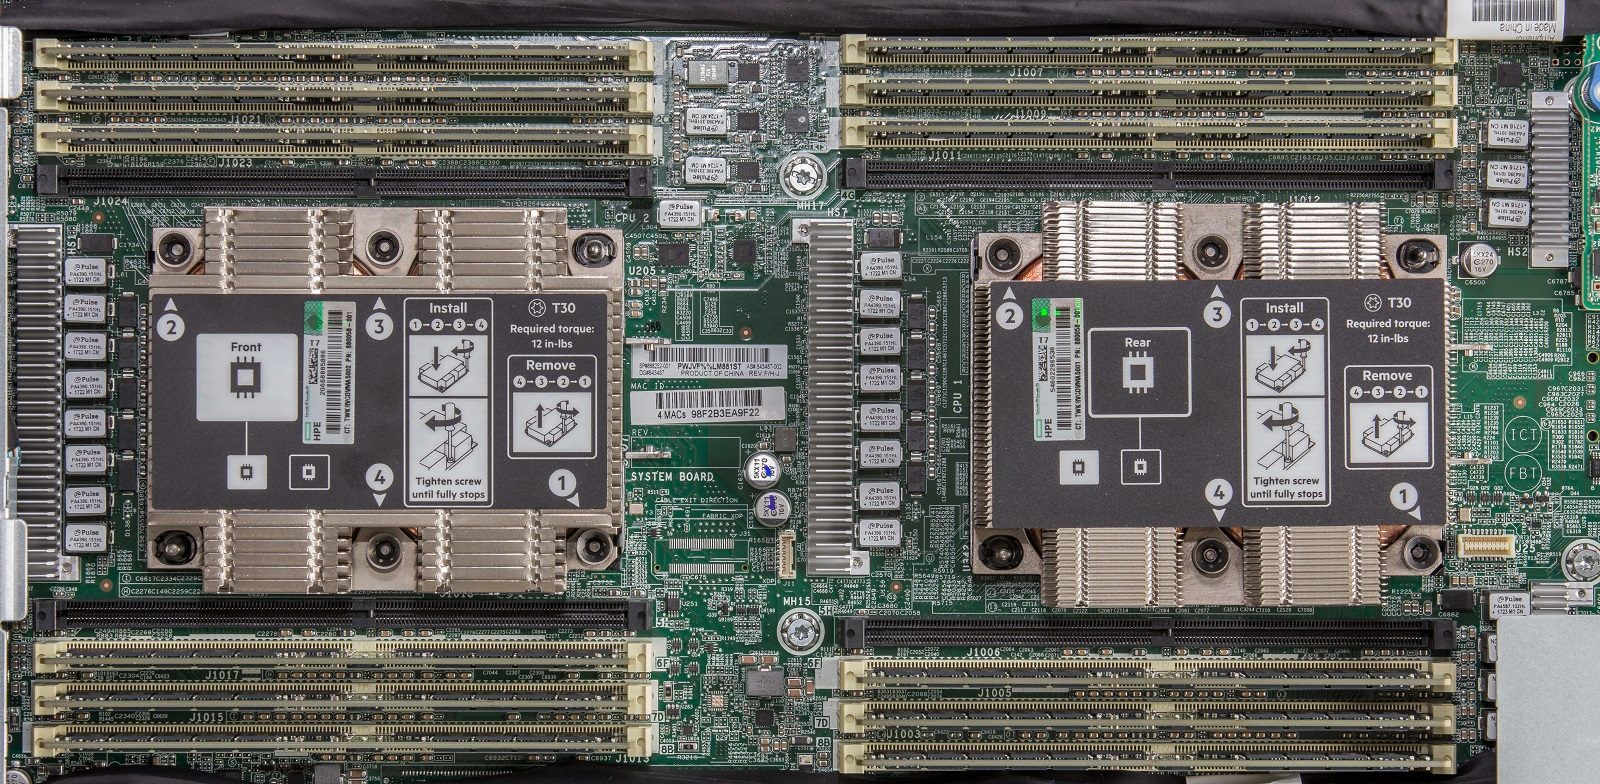
\includegraphics[width=.9\linewidth]{images/motherboard.jpg}
                        \caption{\label{fig:motherboard}Carte mère d'un serveur possédant deux processeurs.}
                    \end{subfigure}\hfill
                \begin{subfigure}[t]{0.48\textwidth}
                        \centering
                        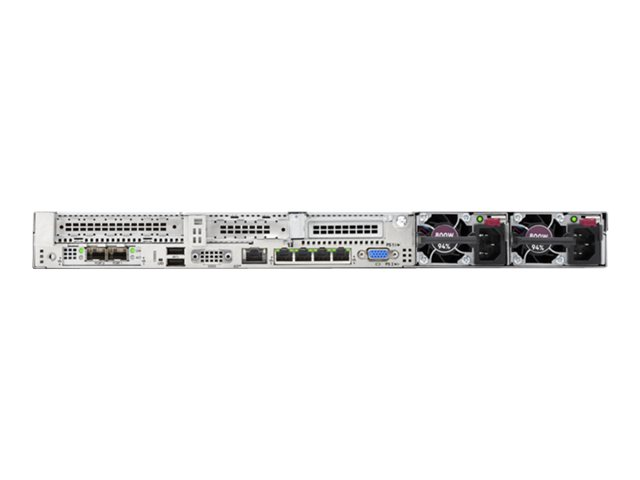
\includegraphics[width=\linewidth]{images/dl360_back.jpg}
                        \caption{Vu arrière d'un serveur exposant les différentes interfaces de connexion.\label{fig:dl360_back}}
                    \end{subfigure}
                    \caption{Exemple d'un serveur utilisé dans les supercalculateurs.}
                    \label{pic_pi_rect}
                \end{figure}
    
            \item \textbf{Les accélérateurs}. Un principe fondamental des processeurs énoncés par Von Neumann était leur universalité. Leur faculté à exécuter tout type de code est à la fois une force, mais aussi un de leur plus grande faiblesse. Ils sont très peu efficaces, en temps et en énergie, pour résoudre certains types de calculs tels que les traitements de signaux ou d'objets géométriques. Pour certaines classes de problème, les supercalculateurs ont recours à des architectures spécialisées appelées accélérateurs:
                \begin{itemize}
    
                    \item\textbf{Les GPU}. À l'origine, les \gls{gpu} étaient destinés au domaine des jeux vidéo et aux calculs de rendus graphiques. Suite à leur utilisation pour d'autres applications que le rendu graphique, ces accélérateurs sont aussi nommés GP-GPU pour \textit{general purpose GPU}. À l'inverse des processeurs, les GPU sont composés de nombreux coeurs (plusieurs centaines). Ceux-ci sont moins complexes et performants que les coeurs de processeur, mais leur nombre les rend particulièrement efficaces pour certaines applications. La \autoref{fig:CPUvsGPU} compare l'évolution des performances des GPU avec celles des CPU de même génération. On remarque l'écart significatif séparant leur performance. Cependant, la figure représente la performance théorique des architectures et il est rare que les applications s'en approchent. 
                    Actuellement, il existe deux fournisseurs principaux de GPU (Nvidia et AMD) qui ont pu bénéficier de leur longue expérience dans le domaine du jeu vidéo. La première nécessite l'utilisation de langage propriétaire (\verb|CUDA|) quand la deuxième peut être programmée grâce au langage \verb|OpenCL|. Le principal avantage de \verb|CUDA| est de pouvoir utiliser des librairies optimisées par NVIDIA pour ses plateformes pour différents domaines (algèbre linéaire (cuBLAS, CUSPARSE), analyse de signal (cuFFT), apprentissage machine (cuDNN, TensorFlow)). 
                    \verb|OpenCL| a été initié par Apple et est maintenant maintenu par le groupe Khronos. C'est un standard ouvert et libre de droits permettant l'exécution de codes sur différentes plateformes. Une application utilisant \verb|OpenCL| pourra être, en théorie, facilement portée sur d'autres architectures (CPU, FPGA, DSP). 
                    
                        \begin{figure}
                        \center
                        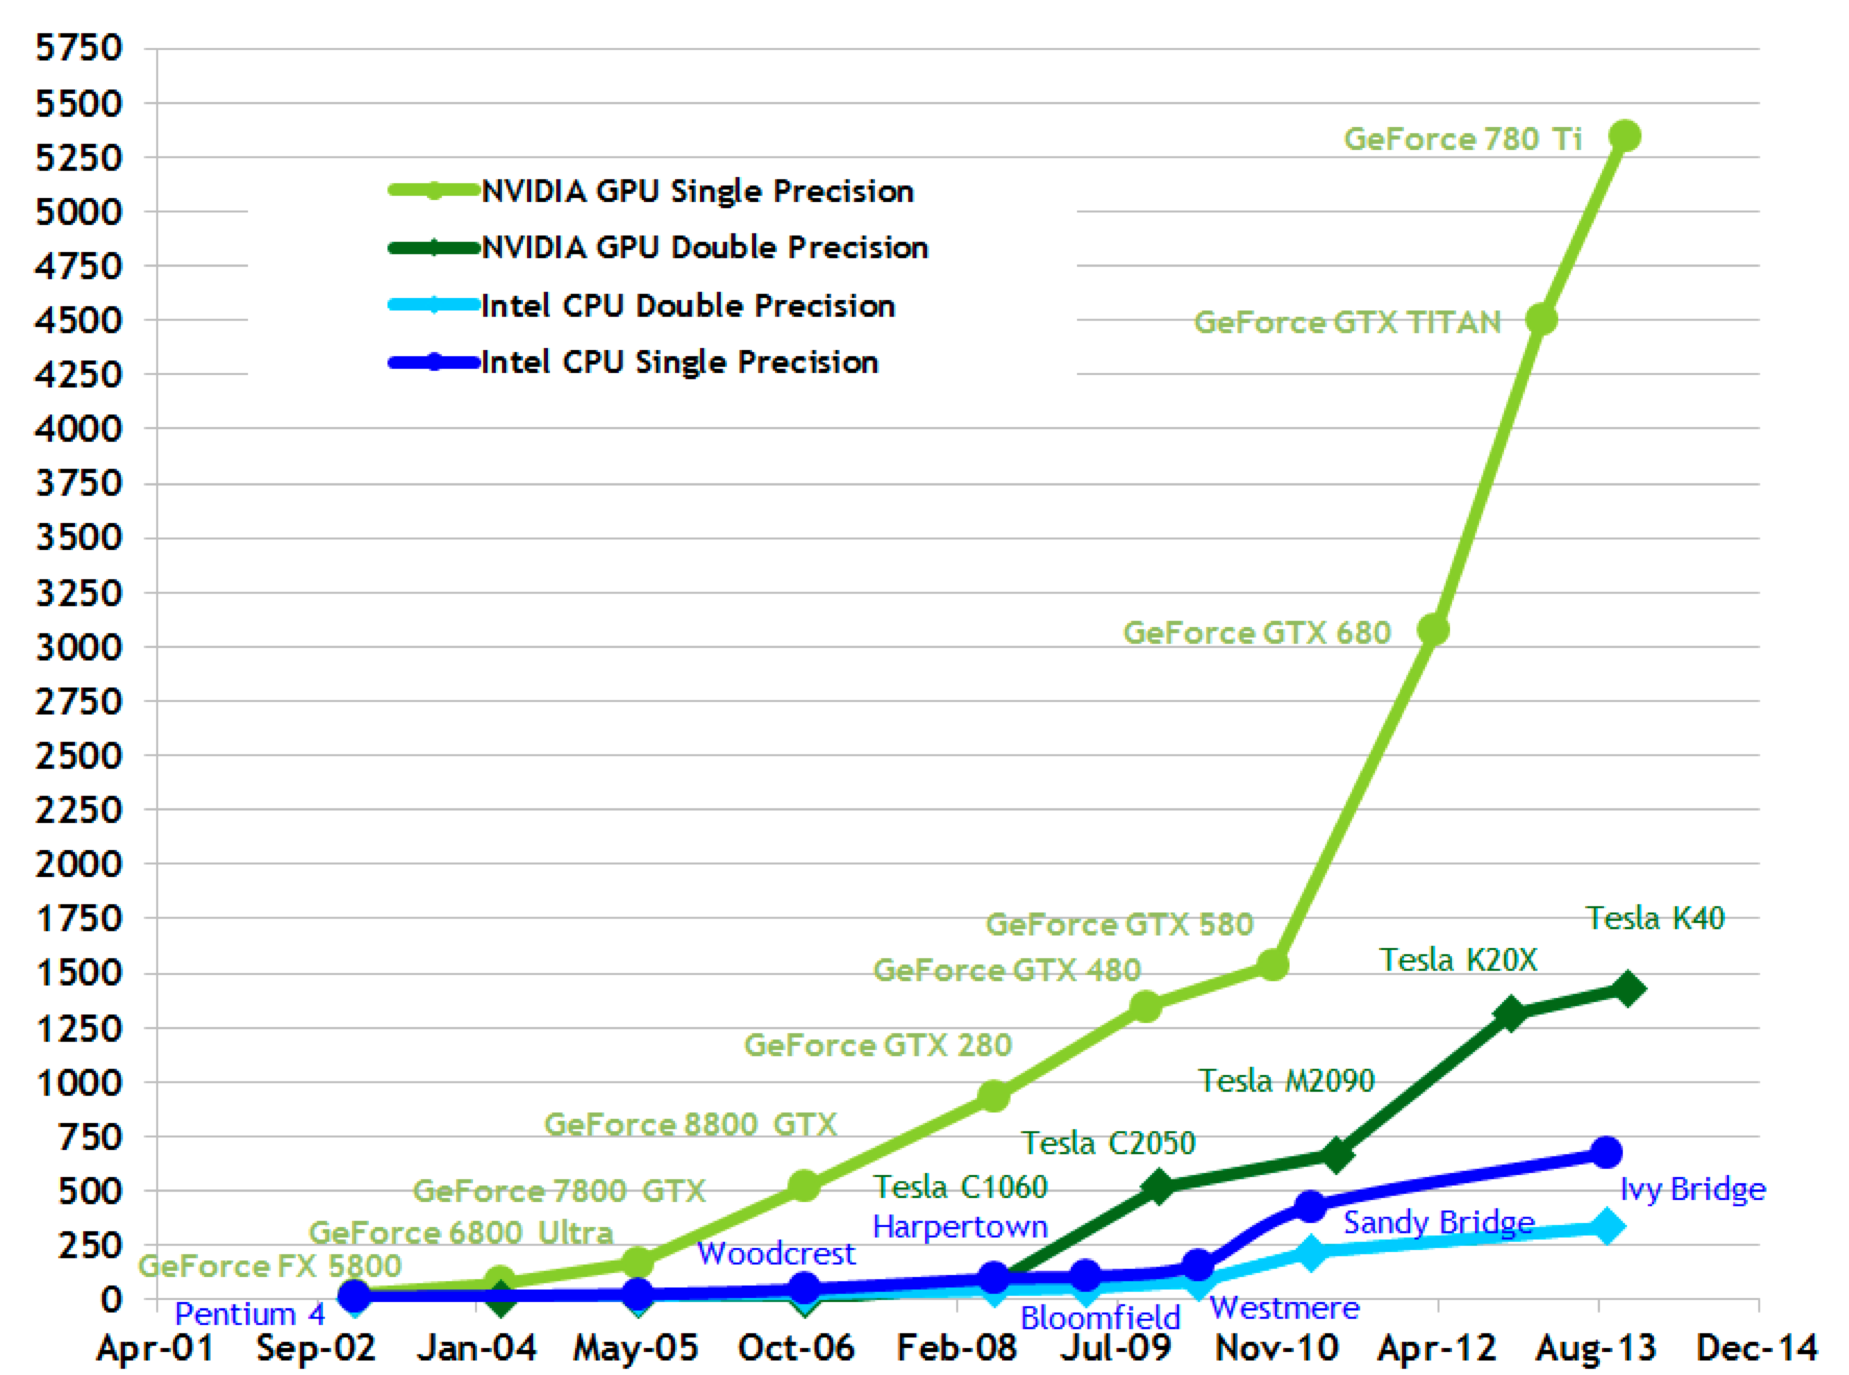
\includegraphics[width=10cm]{images/CPUvsGPU.png}
                        \caption{\label{fig:CPUvsGPU} Comparaison des performances entre différentes générations de CPU et de GPU}
                        \end{figure}
                     
                    
                    
                    
                    %Cependant, pour des applications particulièrement adaptées, le GPU n'a pas d'équivalent actuellement en termes de performance. La performance du bus mémoire d'un GPU est elle aussi bien supérieure, rendant ces architectures d'autant plus intéressantes pour les codes dont la performance est limitée par le système mémoire. 
                    
                    %Acutellement, le développement ou le portage d'applications pour pouvoir être exécutées sur ces architectures demande un investissement conséquent. L'architecture spécifique des GPU nécessite au programmeur de présenter explicitement la parallélisation d'un noyau. De plus, le GPU possédant son propre espace mémoire, le programmeur doit gérer explicitement les transferts entre celle-ci et la mémoire centrale du serveur.
                    %De nombreux travaux essaient de combler cette difficulté. La plus notable étant surement OpenACC. Crée en 2011, cet outil permet d'annoter le code source d'une application à l'aide de \verb|#pragma| pour indiquer au compilateur les zones parallélisable. Avec un effort raisonable, des performances proches des performances atteinte en utilisant \verb|CUDA| peuvent être atteinte. 
                        
                            
                    \item\textbf{Les FPGA.}  Les \gls{fpga} sont de simples circuits intégrés qui contiennent des portes logiques pouvant être programmées pour la réalisation d'un circuit. 
                    Les méthodes traditionnelles de développement sur FPGA nécessitent la conception d'une architecture matérielle utilisant un langage dédié (Hardware Description Language (HDL)). Pour ce faire, le développeur doit concevoir les chemins de données ainsi que la logique de contrôle. Il s'agit d'un processus de développement fastidieux et complexe qui peut entraver leur adoption. Les FPGA les plus récents peuvent être programmés à l'aide d'\verb|OpenCL|.
                    Implémenter un circuit à l'aide d'un FPGA peut fournir une efficacité énergétique légèrement inférieur à celle obtenue par une implémentation d'un \gls{asic}. Cependant, le fait que les FPGA soient programmables leur donne un avantage sur les ASIC, car le même matériel peut être reprogrammé en un nouveau circuit. Le temps de reprogrammation étant relativement faible, il peut être intéressant de reprogrammer le FPGA plusieurs fois pour les différentes phases de l'application. Cependant, la complexité de programmation des FPGA et leur prix très élevé sont les principaux freins pour leur adoption dans les supercalculateurs.        
                    
                    \item\textbf{Les DSP}. Les \gls{dsp} sont adaptés pour les opérations de convolution et de filtrage très utilisés par les algorithmes d'analyse de signal. Généralement contraints par leur consommation électrique (matériel embarqué, smartphone, robotique), les DSP utilisent des fréquences plus basses que les processeurs. Du fait de leur implémentation d'opérations optimisées, elles sont plus efficaces que les architectures standards pour ces applications. Les opérations de filtrage nécessitent, pour être optimales, d'avoir accès à chaque cycle à une instruction et deux opérandes. Les architectures Harvard (voir \autoref{sec:harvard}) sont alors plus optimales pour ce type d'exécution grâce à leurs deux bus d'accès (données et instructions).
                     
             \end{itemize}
             
             
                %Étant architecturalement adaptés à certains algorithmes, les accélérateurs sont généralement plus efficaces énergétiquement. Dans un contexte où l'énergie est une pression majeure, leur utilisation est d'autant plus pertinente. Pour pouvoir être utilisées et obtenir les meilleures performances, les applications doivent être adaptées. Cela impose aux développeurs d'apporter des transformations à leur code, d'utiliser un nouveau compilateur ou même un autre langage. Ces transformations peuvent réduire la portabilité de l'application, notamment quand un langage propriétaire, tel que \verb|CUDA| est utilisé.  Un accélérateur peut être adapté à la résolution d'une partie de l'application, mais peut être très inefficace pour le reste. Cela rend le choix de l'accélérateur difficile, car l'investissement (budget et modification de code) doit être rentable pour l'utilisateur.
           
                  
                    
            \item \textbf{Le stockage}. Les applications de calculs intensifs ont besoin d'avoir accès à une grande capacité de stockage. Certaines applications utilisent des jeux de données dépassant de plusieurs facteurs la capacité de stockage du serveur. Ceux-ci doivent donc être stockés à l'extérieur du serveur. D'autres applications peuvent produire des résultats ne pouvant pas non plus être stockés sur les serveurs. Pour ces deux utilisations, un supercalculateur doit posséder un stockage avec les meilleures caractéristiques possible: latences, débits, fiabilité. Suivant le type d'application, la priorité n'est pas la même.
            
            
                   
            \item \textbf{L'interconnexion}\label{sec:edl_interco} Les applications étant réparties sur différents serveurs, ces derniers ont besoin d'être interconnectés pour s'échanger des informations (résultats temporaires, instructions) ou pour se synchroniser. Le système d'interconnexion participe à une part importante de la performance finale. Le matériel utilisé doit donc être adapté aux besoins de l'application. Suivant sa nature, une application bénéficie d'un réseau avec une faible latence et/ou un débit élevé.
            La latence inclut le temps nécessaire aux routeurs pour rediriger le message au destinataire. Pour cela, la structure des routeurs doit être bien pensée pour réduire le nombre de \textit{sauts} de chaque échange, c'est-à-dire le nombre d'intermédiaires pour aller de l'expéditeur au destinataire. La figure \ref{pic_topologie} montre un exemple de topologie et l'impact qu'elle a sur la latence des communications qui peut être multipliée par deux suivant le destinataire du noeud $A$. Cette structure (ou topologie) doit s'assurer d'éviter tout risque de congestions afin qu'une partie de réseau ne soit pas trop sollicitée ce qui créerait des baisses de performances.    
            Différentes technologies sont ainsi développées pour répondre aux différents besoins (et différents budgets). Les technologies dites \verb|10GbE| (\textit{10 Gigabit Ethernet}), basées sur TCP, permettent d'échanger des informations pour un débit allant jusqu'à 10 Gb/s. Ce réseau peut être implémenté à l'aide de câble en cuivre ou de fibre optique. Un second protocole appelé Infiniband permet d'atteindre des débits plus élevés tout en assurant la réussite des transferts. En fonction de l'application utilisée, le choix de la technologie réseau utilisée peut avoir un fort impact sur ses performances \cite{Council2009}.
                Aussi, l'efficacité du réseau ne dépend pas seulement du matériel, la partie logiciel est tout aussi importante comme la complexité des protocoles ou la performance des algorithmes de routage.
                
                    \begin{figure}
                    \center
                    \includegraphics[width=6cm]{images/Chapitre1/TopologieReseau.png}
                    \caption{\label{pic_topologie} Exemple d'une topologie d'un cluster. Si le serveur A veut envoyer un message à B, il devra effectuer 4 sauts (ou \textit{hop}).}
                    \end{figure}
          
    
            \item \textbf{Le système de refroidissement}. La puissance électrique utilisée par les différents matériels est dissipée sous forme de chaleur. Il n'est pas rare qu'une armoire (un \textit{rack}) consomme à elle toute seule plus de 50 kW. Un supercalculateur doit donc posséder un système de refroidissement performant pour éviter les surchauffes des composants. En effet, celles-ci peuvent provoquer un ralentissement des matériels (fréquences des processeurs) ou même les détériorer. De nombreuses technologies ont été développées pour améliorer le rendement des systèmes de refroidissement tels que le refroidissement liquide ou l'immersion des composants dans des bains d'huile.
        \end{enumerate}


\subsection{Programmation parallèle et performance des supercalculateurs}      
\label{sec:prog_parallele}
%%%%%%%%%%%%%%%%%%%%%%%%%%%%%%%%%%%%%%%%%%%%%%%%%%%%%%%%%%%%%%%%%%%

    \subsubsection{Le calcul parallèle}\label{sec:exemple_pi}
    %%%%%%%%%%%%%%%%%%%%%%%%%%%%%%%%%%%%%%%%%%%%%%%%%%%%%%%%%%%%%%%%%%%
        
        L'agrégation de milliers de ressources de calcul (processeurs, accélérateurs) a pour objectif d'accélérer l'exécution d'applications qui ne pourraient pas être réalisées par une seule d'entre elles dans un temps raisonnable. Le travail des programmeurs est alors de diviser ce problème complexe en sous-problèmes indépendants, pouvant être résolus simultanément par les différentes ressources. Cette méthode de résolution, appelée calcul parallèle, regroupe l'ensemble de moyens, logiciels et matériels qui permettent de réduire le temps de calcul d'un programme en répartissant la charge de travail.
       
        Pour illustrer la nécessité d'avoir recours aux techniques de calcul parallèle, nous présentons un exemple simple permettant de réaliser l'approximation de $\pi$ par le calcul de l'intégrale suivante:
        \begin{equation}
        \label{eq_pi}
        \int_{0}^{1} \frac{4.0}{1 + x^{2}}
        \end{equation}
        
        %ILLUSTRATION PI    
        \begin{figure}[t!]
            \centering
            \begin{subfigure}[t]{0.5\textwidth}
                \centering
                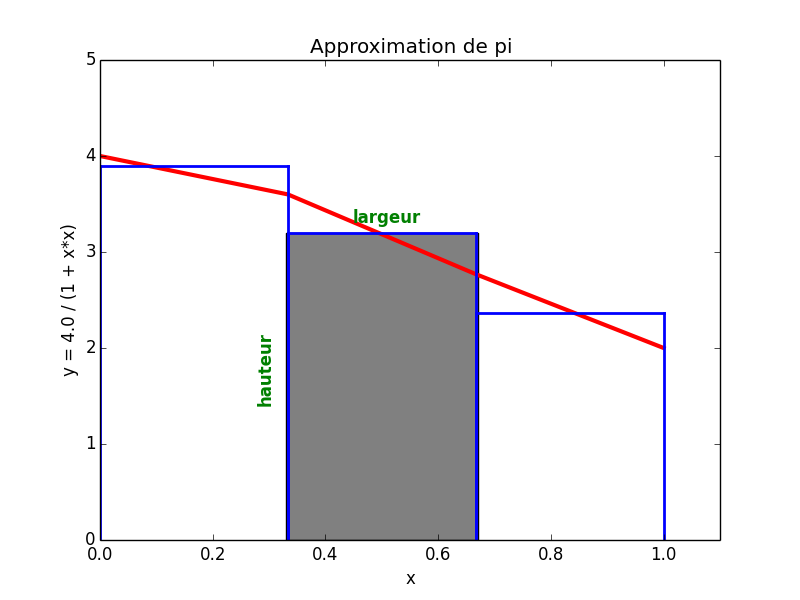
\includegraphics[height=2.2in]{images/Chapitre1/pic_pi_rect_1.png}
                \caption{\label{pic_pi_1} Approximation avec 4 rectangles}
            \end{subfigure}%
        \begin{subfigure}[t]{0.5\textwidth}
                \centering
                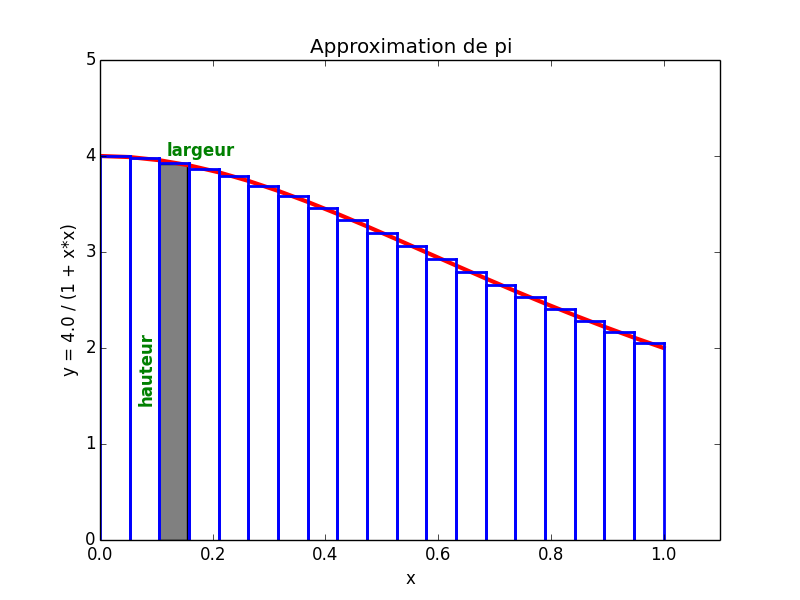
\includegraphics[height=2.2in]{images/Chapitre1/pic_pi_rect_2.png}
                \caption{Approximation avec 14 rectangles}
            \end{subfigure}
            \caption{\label{pic_pi_2} Méthode des rectangles: exemple de deux exécutions de l'algorithme avec un nombre de rectangles différents.}
            \label{pic_pi_rect}
        \end{figure}
            
        Calculer une intégrale revient à calculer l'aire formée par cette courbe et l'axe des abscisses dans le domaine étudié, ici $[0,1]$. Cette surface peut être approximée par la méthode des rectangles (ou trapèze). Cette méthode revient à dessiner des rectangles sous la courbe (voir \autoref{pic_pi_1}). Leur surface étant calculable, il est alors possible d'approcher l'intégrale donnée dans l'\autoref{eq_pi} à l'aide du code présenté dans l'extrait de code suivant:
        
        %ALGO PI
        \begin{lstlisting}[language=C, caption=Implémentation de l'algorithme de calcul d'intégrale par la méthode des rectangles, float,floatplacement=H]
double x, largeur, hauteur, pi = 0.0;

int num_steps = 4;
int num_steps = 14;

largeur = 1.0 / num_steps;

for (int i = 0; i < num_steps; ++i) {
    x =  (i) * largeur;
    hauteur = ( 4.0/(1.0+x*x));
    pi += largeur * hauteur;
}

cout << "Valeur de pi: " << pi << endl;
\end{lstlisting}
    
         Nous remarquons sur la \autoref{pic_pi_1}, qu'avec l'utilisation de quatre rectangles, la surface des rectangles ne correspond pas exactement à la courbe à approcher. Ces erreurs affectent la précision de notre programme qui affiche une valeur de $\pi = 3.38$. La \autoref{pic_pi_2} présente le même programme qui utilise 14 rectangles. Les rectangles sont alors plus fidèles à la courbe et le programme calcule une valeur de $\pi = 3.21$.
        Nous présentons cet exemple simpliste pour illustrer le besoin de puissance de calcul pour réaliser des simulations précises:
        \begin{itemize}
            \item La précision du calcul dépend du nombre de rectangles choisi. Plus le nombre de rectangles utilisés est grand, plus la précision augmente. Cependant, augmenter le nombre de rectangles à calculer augmente le nombre d'opérations nécessaires à réaliser. 
            
            \item Pour accélérer le calcul de cette application, le calcul des différents rectangles doit être réparti entre les ressources de calcul. À la fin de l'exécution, un processus s'occupe de récolter et additionner les différents résultats.
            
            \item La capacité d'une application à utiliser des ressources parallèles n'est pas automatique. Une transformation du code doit être réalisée de manière explicite (par le programmeur) ou implicite (par le compilateur).
        \end{itemize}
        
    \subsubsection{Niveau de parallélisme des supercalculateurs}
    %%%%%%%%%%%%%%%%%%%%%%%%%%%%%%%%%%%%%%%%%%%%%%%%%%%%%%%%%%%%%%
    
        La performance d'une application parallèle dépend donc du nombre et de la performance des ressources pouvant travailler simultanément pour la résolution du problème. La tâche des programmeurs est d'adapter le code pour répartir l'application sur les différentes ressources disponibles. Ce travail est difficile, car le parallélisme est présent à plusieurs niveaux dans un supercalculateur.
        
        
        \paragraph{Taxonomie de Flynn.}
             Les différentes formes de parallélisme ont été regroupées en quatre classes appelées taxonomie de Flynn \cite{Flynn2011} (voir \autoref{fig:flynn}). Ces classes permettent de caractériser les architectures en fonction de l'indépendance ou non des instructions et des données. La classe \verb=SISD= représente les architectures classiques n'exécutant qu'une instruction sur une donnée à la fois. 
            La classe \verb=SIMD= regroupe les architectures vectorielles exécutant une instruction sur plusieurs données à la fois (voir \autoref{sec:cpu_vectoriel}). La classe \verb|MIMD| représente des architectures exécutant plusieurs instructions sur plusieurs données à la fois. Un serveur possédant plusieurs processeurs est un exemple d'architecture \verb|MIMD|. La dernière classe d'architecture \verb|MISD| exécute des instructions différentes sur le même jeu de données. Les processeurs capables d'exécuter des instructions fusionnées telles que les FMA peuvent être considérées comme telles. Une instruction FMA permet de réaliser une addition et une multiplication sur une même donnée. Le processeur ASIC présent dans les voitures connectées peut par exemple exécuter deux algorithmes différents pour s'assurer de la validité d'une décision à prendre. 
            
            \begin{figure}
            \center
            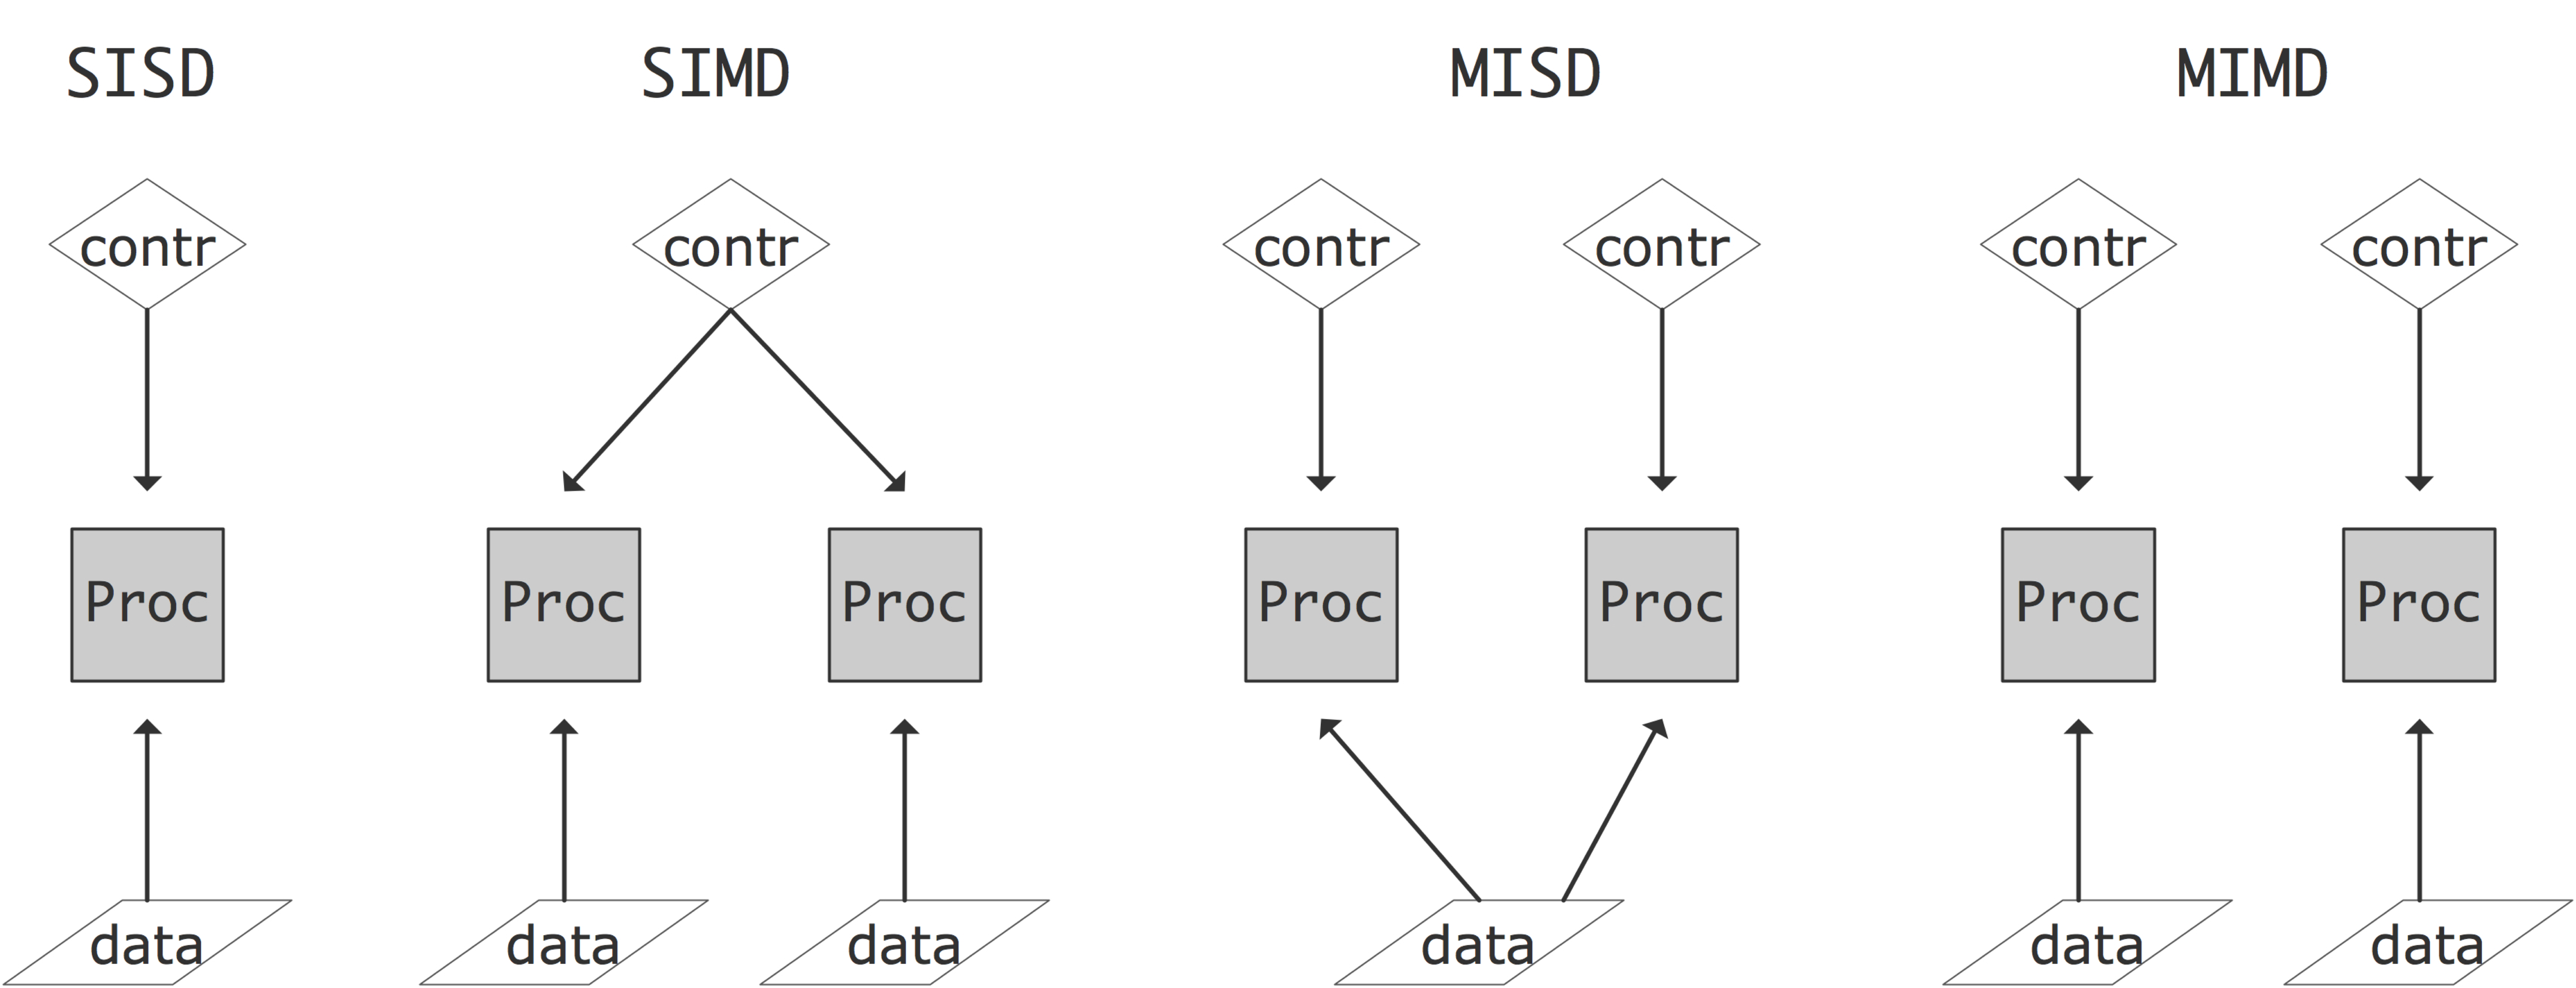
\includegraphics[width=12cm]{images/flynn.png}
            \caption{\label{fig:flynn} Les quatre classes de la taxonomie de Flynn (graphique extrait de \cite{Eijkhout2013})}
            \end{figure}
            

        \paragraph{Niveaux de parallélisme d'un supercalculateur.}
            La \autoref{fig:parallele_hpc} représente les principaux niveaux de parallélisme d'un supercalculateur. Le  niveau $1$ concerne les serveurs, reliés par un système d'interconnexion. Différentes tâches peuvent être assignées à chaque noeud qui peuvent communiquer entre eux pour se synchroniser ou partager des résultats. Le niveau $2$ concerne le parallélisme des processeurs (ainsi que des accélérateurs si le serveur en possède). En fonction des tâches à réaliser et des caractéristiques des ressources de calculs, les tâches peuvent être réparties pour être exécutées. Le niveau $3$ est situé dans les processeurs et concerne l'utilisation de processeurs multicoeurs. Le niveau $4$ est lié aux processeurs superscalaires possédant plusieurs pipelines (voir \autoref{sec:pipeline}). Le dernier niveau de parallélisme concerne les unités de calcul vectorielle des processeurs qui peuvent exécuter une instruction sur plusieurs données simultanément (voir \autoref{sec:fpu}).
            
            \begin{figure}
                \center
                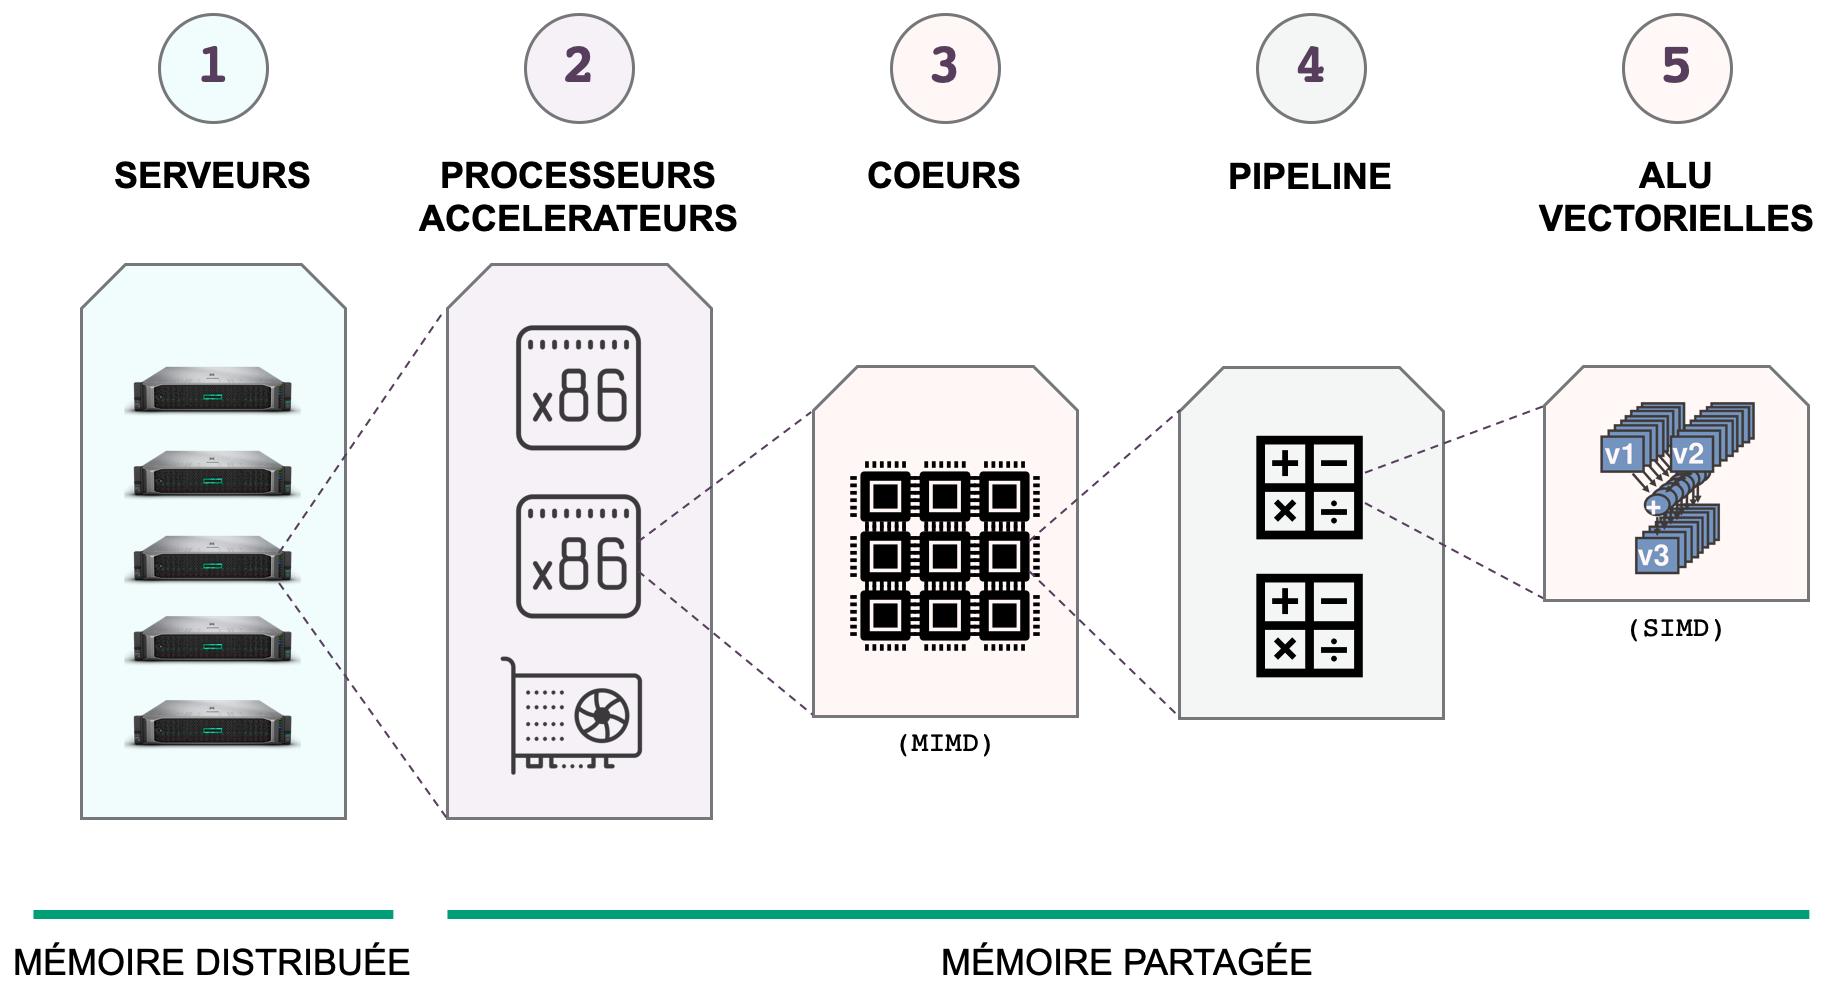
\includegraphics[width=14cm]{images/parallele_hpc.png}
                \caption{\label{fig:parallele_hpc} Différents niveaux de parallélisme dans un supercalculateur.}
            \end{figure}
            
            Pour maximiser le nombre d'instructions pouvant être exécutées sur un supercalculateur (\textit{Instruction Level Parallelism} (ILP)) différentes méthodes existent. Le plus haut niveau consiste à exécuter des applications indépendantes permettant de saturer l'utilisation de la plateforme (\textit{Job Level Parallelism}). Une même application peut être découpée en tâches qui peuvent être exécutées en parallèle (\textit{Task Level Parallelism} (TLP) \cite{Kambadur2009}). Lorsque la nature du code le permet, une instruction peut être exécutée sur plusieurs données simultanément (\textit{Data Level Parallelism}(DLP) \cite{Espasa1997}).

    \subsubsection{Paradigme de programmation}
    %%%%%%%%%%%%%%%%%%%%%%%%%%%%%%%%%%%%%%%%%%%%%%%%%%%%%%%%%%%%%%
       
        Pour pouvoir bénéficier des ressources de calculs disponibles, le programmeur doit adapter certaines parties du code. Les niveaux de parallélisme les plus bas (pipeline et ALU) sont gérés par le matériel sans intervention de l'utilisateur. Par exemple, lorsque le compilateur génère des instructions vectorielles, l'unité de calcul s'occupe seule de leur exécution. Cependant, le programmeur doit connaître les détails de la microarchitecture pour développer du code pouvant tirer parti du parallélisme, par exemple en présentant les instructions permettant au module d'exécution dans le désordre (\autoref{sec:out_of_order}) d'optimiser l'utilisation des pipelines présents dans les processeurs superscalaires.
        
        Pour bénéficier des niveaux $1$, $2$ et $3$ (voir \autoref{fig:parallele_hpc}), deux paradigmes fondamentaux de la programmation parallèle peuvent être utilisés: la programmation à mémoire partagée ou à mémoire distribuée. La principale distinction entre ces deux paradigmes est le partage ou non d'un espace mémoire entre les ressources utilisées (voir \autoref{fig:edl_ditribue_partage}). 
        
            \begin{figure}
                \center
                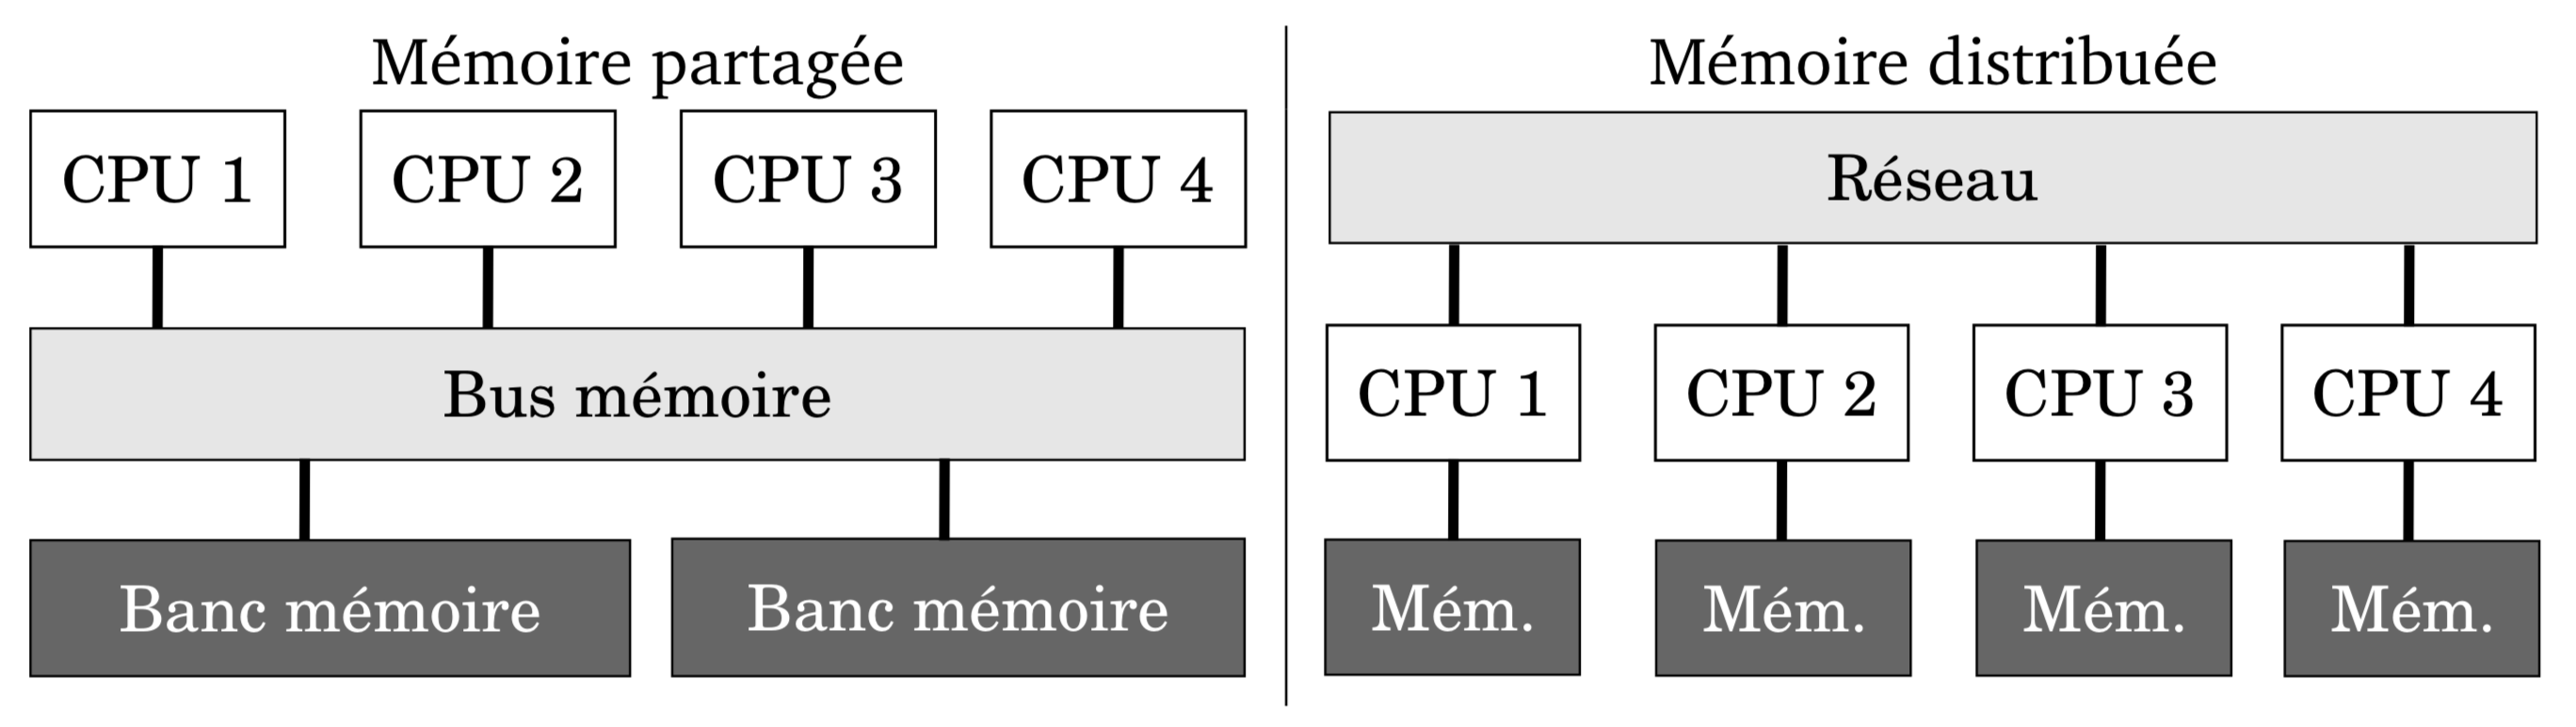
\includegraphics[width=14cm]{images/edl_ditribue_partage.png}
                \caption{\label{fig:edl_ditribue_partage} En fonction de l'architecture et du mode d'accès mémoire, deux paradigmes de programmations peuvent être utilisés (graphique extrait de \cite{Valat2016}).}
            \end{figure}
        
        
        
            
        \paragraph{Programmation à mémoire distribuée.}  
               
            Le paradigme de programmation à mémoire distribuée doit être utilisé lorsque les différents processus n'ont pas accès au même espace mémoire. Les communications entre les ressources de calculs sont alors réalisées par le système d'interconnexion. L'avantage de telles architectures est de permettre d'agréger plus ou moins de ressources en fonction du besoin d'un utilisateur. La performance de la solution est alors dépendante du nombre de serveurs utilisés et permet une plus grande flexibilité. 
            
            Les données nécessaires pour les calculs ainsi que les résultats temporaires doivent être explicitement transférés par l'utilisateur. Pour cela, les programmeurs peuvent utiliser des librairies de \textit{passage de messages}, dont le standard le plus utilisé est une \gls{mpi}. Le standard définit la sémantique des différentes fonctions, identifie les tâches distribuées et propose des moyens d'échange et de synchronisation entre les processus. Le standard est implémenté par des librairies telles que \verb|OpenMPI|, \verb|MPICH-2| ou encore \verb|IntelMPI|. Chaque noeud ayant son propre système d'exploitation, les librairies doivent être installées sur tous les serveurs utilisés. 
        
            La principale difficulté de ce paradigme de programmation est la nécessité de réaliser explicitement les mouvements de données entre les noeuds. L'exécution d'une application peut alors être résumée en 3 étapes. La \autoref{fig:scatter_gather} présente l'étape 1 et 3 d'un programme de calcul à mémoire distribuée:
            \begin{enumerate}
                \item La première étape consiste à répartir le jeu de données à l'aide d'opérations de type \textit{scatter} (voir \autoref{fig:scatter}). 
                \item La deuxième étape est la réalisation du calcul par chaque ressource. Cette étape utilise le paradigme de programmation à mémoire partagée (voir \autoref{sec:prog_partagee}).
                \item Lorsque chacune d'entre elles a terminé son calcul, des opérations de type \textit{gather} (voir \autoref{fig:gather}) permettent de récolter l'ensemble des résultats partiels, pour calculer le résultat final.
            \end{enumerate}
            Les étapes 1 et 3 utilisent le système d'interconnexion du supercalculateur. La performance de celui-ci peut fortement impacter celle des applications. Cette particularité est à l'origine de nombreuses erreurs et rend la programmation à mémoire distribuée difficile. Le programmeur doit avoir à sa disposition des outils lui permettant de suivre l'évolution de chaque phase pour déceler des problèmes de synchronisation ou de déséquilibre de charge.
        
        
            \begin{figure}[t!]
                \centering
                \begin{subfigure}[t]{0.48\textwidth}
                    \centering
                    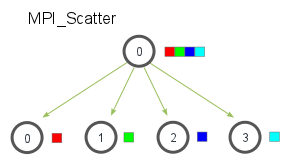
\includegraphics[width=.8\linewidth]{images/scatter.png}
                    \caption{\label{fig:scatter}Les opérations de \textit{scatter} permettent de répartir un jeu de données entre les ressources.}
                \end{subfigure}\hfill
            \begin{subfigure}[t]{0.48\textwidth}
                    \centering
                    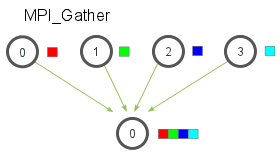
\includegraphics[width=.8\linewidth]{images/gather.png}
                    \caption{\label{fig:gather}Chaque ressource renvoie son résultat local pour calculer le résultat final du calcul.}
                \end{subfigure}
                \caption{\label{fig:scatter_gather}Les deux opérations principales de MPI permettent de répartir et récolter les données entre les différentes ressources participant à la résolution\protect\footnotemark.}
            \end{figure}
            \footnotetext{Source des graphiques - \url{https://mpitutorial.com/tutorials/mpi-scatter-gather-and-allgather/}}
               
               
           
        %%%%%%%%%%%%%%%%%%%%%%%%%%%%%%%%%%%%%%%%%%%%%%
        \paragraph{Programmation à mémoire partagée.} \label{sec:prog_partagee}
            
            Lorsque toutes les ressources de calculs ont accès au même espace mémoire, il est conseillé d'utiliser le paradigme de programmation à mémoire partagée. Comme il n'est plus utile de transférer les données explicitement entre les ressources de calcul, il est possible d'utiliser des \gls{thread} (processus légers). Pour profiter des niveaux de parallélisme $2$ et $3$ (voir \autoref{fig:parallele_hpc}) les programmeurs peuvent avoir recours à des librairies ou même des langages spécifiques aux processeurs ciblés. Pour les processeurs, des librairies telles que \verb|OpenMP| ou \verb|Pthread| sont utilisées pour accéder au niveau $3$ de parallélisme qui consiste à répartir l'application sur les différents coeurs. Les accélérateurs de type GP-GPU peuvent être programmés à l'aide d'\verb|OpenCL| ou de \verb|CUDA|. Ces librairies sont basées sur le modèle de programmation \verb|fork/join| (voir \autoref{fig:openmp}). Lorsqu'une partie du code doit être exécutée en parallèle, le thread \textit{maître} se dédouble (\textit{fork}) en plusieurs threads pouvant être exécutés indépendamment sur différents coeurs. Une fois les tâches réalisées, les threads sont arrêtés et le programme continue son exécution séquentiellement. Ce modèle de programmation utilisant la même mémoire partagée, le programmeur doit veiller à ce que les différents threads utilisent des données en commun. Un avantage d'\verb|OpenMP| est sa facilité d'utilisation pour exprimer le parallélisme depuis le code source de l'application. À l'aide de directives préprocesseur, les zones exécutables en parallèle doivent être annotées à l'aide de \verb|#pragma|. Différentes options permettent de définir le nombre de threads à générer, la façon de partager le travail ou encore définir le mode d'accès aux données (partagé, privé). Le code listé dans l'\autoref{lst:openmp} permet de répartir les différentes itérations d'une boucle (indépendantes) entre les threads.
            
\begin{lstlisting}[language=C, caption=Distribution des itérations d'une boucle à l'aide d'OpenMP, label=lst:openmp]
#pragma omp parallel for
for (i=0;i<20;i++)
    a[i]=b[i] + 42;
\end{lstlisting}

                \begin{figure}
                \center
                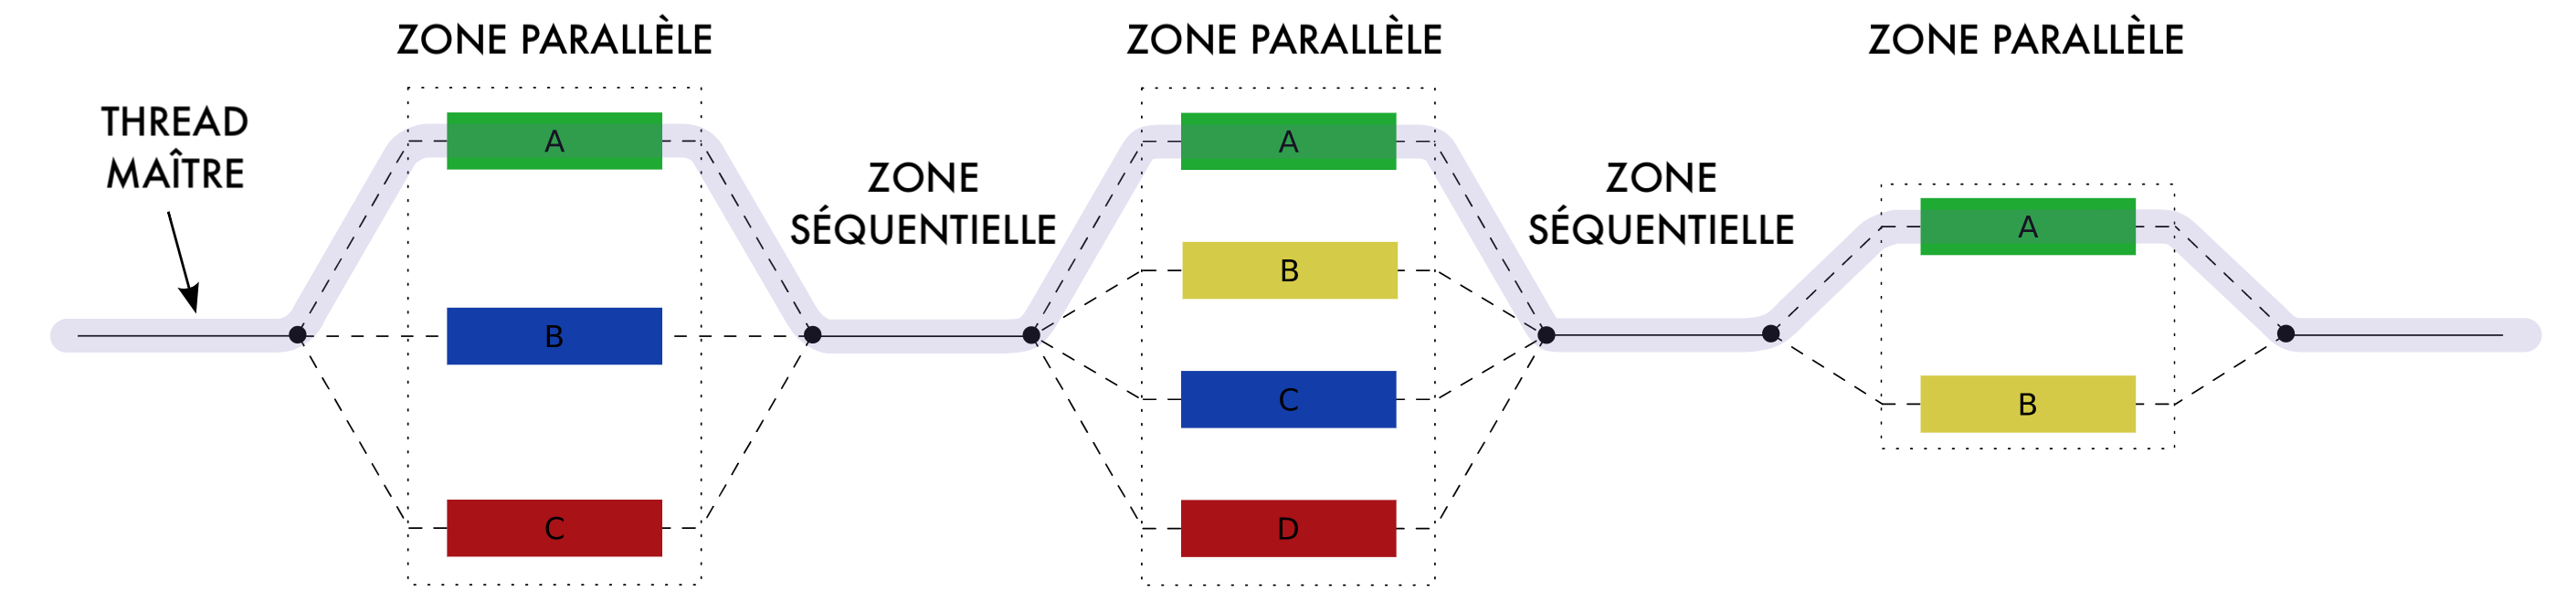
\includegraphics[width=14cm]{images/openmp.png}
                \caption{\label{fig:openmp} Pour accéder au parallélisme des coeurs, OpenMP crée des \textit{threads} indépendants\protect\footnotemark.}
                \end{figure}
                \footnotetext{Graphique adapté de \url{https://en.wikipedia.org/wiki/Fork\%E2\%80\%93join_model}}
                

\subsection{Performance de la parallélisation}
\label{sec:parallele_perf}
%%%%%%%%%%%%%%%%%%%%%%%%%%%%%%%%%%%%%%%%%%%%%%%%%%%%%%%%%%
    
        L'utilisation d'un supercalculateur a pour objectif d'accélérer l'exécution d'une application. Cette accélération peut alors permettre d'obtenir des résultats plus rapidement ou bien d'étudier des problèmes plus complexes. L'accélération d'une application, notée $Speedup(P)$, correspond au rapport entre le temps nécessaire pour exécuter l'application sur une ressource unique (noté $T_{sequentiel}$) et le temps nécessaire lorsque $P$ ressources identiques sont utilisées (noté $T_{parallele}$). L'accélération est dite optimale lorsque le temps de résolution $T_{parallele}(P)$ évolue linéairement avec le nombre $P$ de ressources. On parle alors d'accélération linéaire:
        
        \begin{equation}
        \label{eq_speedup}
        Speedup_{lineaire} (P) = \frac{T_{sequentiel}}{T_{parallele}(P)} = P
        \end{equation}
        
        Prenons l'exemple d'une application dont le temps nécessaire à l'exécution prend  $T_{sequentiel} = 2$ minutes. Une accélération linéaire avec l'utilisation de $P = 4$ processeurs pendrait alors $T_{parallele} = 30$ secondes. En pratique il est très rare d'obtenir une telle accélération, car certaines parties du code ne peuvent pas être parallélisées (transmission des données en programmation à mémoire distribuée, zone critique en programmation à mémoire partagée, synchronisation). 
        Pour évaluer la capacité d'une plateforme à utiliser efficacement les ressources supplémentaires pour l'exécution d'une application, il est courant de mesurer sa scalabilité. La scalabilité d'une application est un indicateur permettant d'évaluer sa capacité à \textit{passer à l'échelle}, c'est-à-dire d'évaluer l'accélération de son exécution lorsque des ressources de calculs supplémentaires sont allouées. On distingue alors deux scalabilités: la forte et la faible (voir \autoref{fig:scaling}). Les résultats des tests de scalabilité forte et faible permettent de choisir un nombre adapté de ressources à utiliser pour une application.
        
            \begin{figure}[t!]
                \centering
                \begin{subfigure}[t]{0.48\textwidth}
                    \centering
                    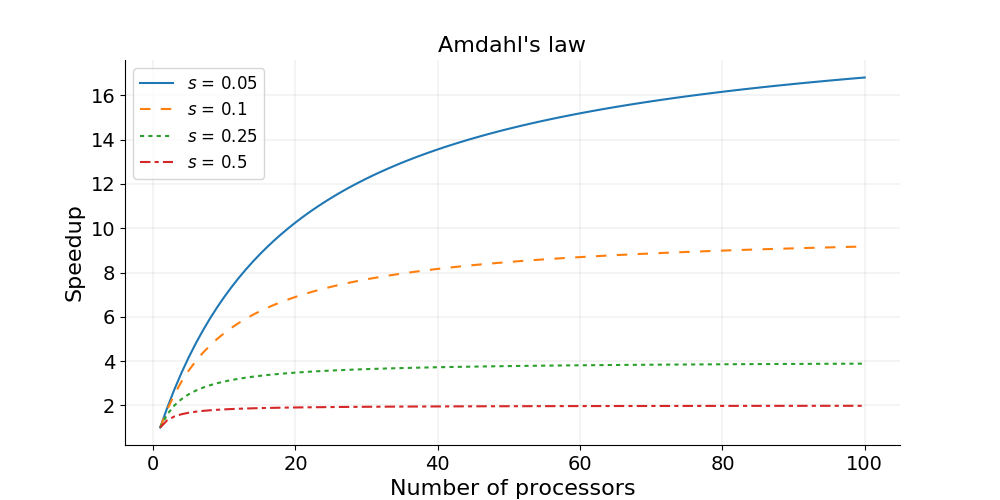
\includegraphics[width=1.05\linewidth]{images/scaling_amdahl.png}
                    \caption{\label{fig:scaling_amdahl}Loi d'Amdahl: la scalabilité forte utilise un problème de complexité constante.}
                \end{subfigure}\hfill
            \begin{subfigure}[t]{0.48\textwidth}
                    \centering
                    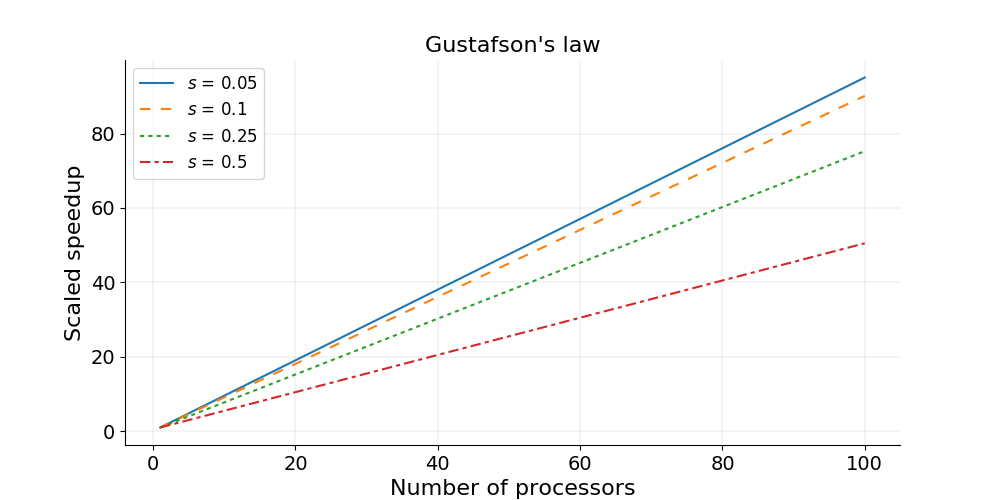
\includegraphics[width=1.05\linewidth]{images/scaling_gustafson.png}
                    \caption{\label{fig:scaling_gustafson}Loi de Gustafson: la scalabilité faible utilise un problème de complexité croissante.}
                \end{subfigure}
                \caption{\label{fig:scaling} Évolution de la scalabilité forte et faible lorsque $P$ processeurs sont utilisé pour l'exécution d'une application ayant une proportion $s$ de code séquentiel\protect\footnotemark.}
            \end{figure}
            \footnotetext{Source des graphiques - \url{https://www.kth.se/blogs/pdc/2018/11/scalability-strong-and-weak-scaling}}
            

    \subsubsection{Scalabilité forte} 
    %%%%%%%%%%%%%%%%%%%%%%%%%%%%%%%%%%
        
        En 1967, l'ingénieur Gene Amdahl a étudié et théorisé l'évolution de l'accélération d'une application avec l'ajout de ressources de calculs, créant ainsi la loi éponyme \cite{Amdahl1967}. La taille du problème étant fixe, chaque unité de calcul a donc moins de travail à réaliser. Idéalement, le temps d'exécution doit être réduit d'un facteur $1/P$ lorsque $P$ ressources sont ajoutées (voir \autoref{fig:scaling_amdahl}). Une application de calcul parallèle n'étant jamais totalement parallélisable, elle possède toujours une proportion de code devant être exécuté séquentiellement. Cette proportion est notée $s$. L'ajout de ressources de calcul n'est alors bénéfique que pour la proportion de code dit parallélisable et noté $1-s$. Le temps nécessaire pour l'exécution de l'application est la somme du temps passé dans la zone séquentielle et de celui passé dans la zone parallèle. En utilisant $P$ processeurs le temps de l'exécution parallèle peut être calculé ainsi: 

        
            \begin{equation}
            T_{parallele}(P) = s \times T_{sequentiel} + \frac{(1-s) \times T_{sequentiel}}{P}
            \end{equation}
        
        L'accélération de l'application peut alors être calculée grâce à l'\autoref{eq_speedup} donnant lieu à l'équation suivante, appelée loi d'Amdahl:
        
                
            \begin{equation}
            \label{eq_amdahl}
            Speedup (P) = \frac{T_{sequentiel}}{s \times T_{sequentiel} + \frac{(1-s) \times T_{sequentiel}}{P}} =  \frac{1}{s + \frac{1-s}{P}}
            \end{equation}
        
        L'accélération d'une application dépend donc du nombre de ressources de calculs supplémentaires allouées à la résolution de l'application, mais aussi de la proportion de zones exécutables en parallèle. La \autoref{fig:scaling_amdahl} montre l'importance de l'influence de la proportion de code séquentiel $s$ sur l'accélération de l'application. Grâce à la loi d'Amdahl, il est possible de donner la limite théorique de l'accélération $Speedup$ d'une application (notée $Speedup_{max}$),  lorsque des ressources de calculs supplémentaires sont utilisées pour la résolution d'un problème de taille fixe. L'accélération maximale d'une application utilisant 95\% de son temps d'exécution dans une fonction entièrement parallélisable peut être calculée par la limite suivante:         
        \begin{equation}
        Speedup_{max} =  \lim_{p\to\infty}    \frac{1}{0.05 + \frac{0.95}{P}} = \frac{1}{0.05} = 20         
        \end{equation}
        Quel que soit le nombre de ressources allouées à l'exécution de cette application, l'application étudiée en exemple ne pourra jamais être accélérée de plus de 20 fois.  
        
        
        %Les coûts engendrés par ces différentes opérations sont notés $T_{couts}$. La durée de l'exécution du programme parallèle peut alors être calculée par la formule suivante:
                %En supposant des coûts $T_{couts}$ associés à l'utilisation du parallélisme, le temps d'exécution du programme parallélisé peut être calculé ainsi:
        %\begin{equation}
        %T_{parallele} = \frac{T_{sequentiel}}{P} + T_{couts}
        %\end{equation}
        
       
    \subsubsection{Scalabilité faible} 
    %%%%%%%%%%%%%%%%%%%%%%%%%%%%%%%%%%
        
        La loi d'Amdahl est très utile pour montrer la nécessité de développer des applications avec la plus grande portion de code parallélisable. Cependant, la loi suppose une taille de problème constante. Lorsque des ressources de calculs supplémentaires sont disponibles, les applications utilisent généralement des jeux de données plus grands pour profiter de l'espace mémoire supplémentaire. La loi d'Amdahl supposant un jeu de donnée fixe n'est alors pas adaptée. Pour y remédier, Gustafson énonça une nouvelle loi en 1988 \cite{Gustafson1988} permettant de prendre cet aspect en considération. 
        Lorsque la taille du jeu de données augmente, la partie séquentielle du programme représente généralement une plus faible portion, car les données sont traitées dans les zones parallèles. Pour une application ayant une proportion de $1-s$ pouvant être exécutée en parallèle sur $P$ processeur, l'accélération peut être calculée par la loi de Gustafson:         
        \begin{equation}
            Speedup (P) = s + (1-s) * P         
        \end{equation}
        
        La scalabilité faible utilise une taille de problème qui évolue à mesure que des ressources supplémentaires sont allouées. Dans ce cas-là, la taille du problème pour chaque unité de calcul est fixe. Dans l'idéal, le temps d'exécution de l'application doit rester constant lors de l'ajout de ressources de calculs (voir \autoref{fig:scaling_gustafson}). Contrairement à la scalabilité forte, l'accélération obtenue par la scalabilité forte n'a pas de limite théorique. 
        
        